\documentclass[10pt]{article}
\usepackage[margin=1in]{geometry}
\usepackage[utf8]{inputenc}
\usepackage{multicol}
\setlength{\columnsep}{1mm}
\usepackage{amsfonts}
\usepackage{booktabs}
\usepackage{siunitx}
\usepackage[authoryear,round]{natbib}
\usepackage{float}
\usepackage[font={small}]{caption}
\usepackage[labelfont=bf]{caption}
\usepackage{lineno}
\usepackage{amsmath,amssymb,setspace,fancyhdr,geometry,url,color}
\usepackage{subfigure,graphicx,caption}
\usepackage{lscape,amsthm}
\usepackage{blindtext}
\usepackage{hhline}
\usepackage{arydshln}
\usepackage{verbatim}
\usepackage{dblfloatfix}
\usepackage{multirow}
\usepackage{graphicx}
\usepackage{xr}

\externaldocument{../PhaseIIPaper/Part1/main1}

\renewcommand\thefigure{S\arabic{figure}}
\renewcommand\thetable{S\arabic{table}}
\renewcommand\thesection{S\arabic{section}}
\setcounter{table}{0}
\setcounter{figure}{0}

%\biboptions{authoryear, comma}
%%%%%%%%%%%%%%%%%%%%%%%%%%%%%%%%%%%%%%%%%%%%%%%%%%%%%%%%%%%%%%%%%%%%%%%%%
%%%%%%%%%%%%%%%%%%%%%%%%%%%%%%%%%%%%%%%%%%%%%%%%%%%%%%%%%%%%%%%%%%%%%%%%%%
\begin{document}
\centering{\bf {\large Supplemental Material} \\
{\Large The GGCMI Phase 2 experiment: global gridded crop model simulations under uniform changes in CO$_2$, temperature, water, and nitrogen levels (protocol version 1.0)}}\\

\vspace{3mm}

\centering{James Franke$^{1, 2}$, 
Christoph M\"{u}ller$^3$, 
Joshua Elliott$^{2, 4}$, 
Alexander Ruane$^5$,  
Jonas J\"{a}germeyr$^{3, 2, 4, 5}$,\\ 
Juraj Balkovic$^{6, 7}$, 
Philippe Ciais$^{8, 9}$, 
Marie Dury$^{10}$, 
Pete Falloon$^{11}$,\\ 
Christian Folberth$^{8}$, 
Louis Fran{\c{c}}ois$^{10}$, 
Tobias Hank$^{12}$, 
Munir Hoffmann$^{13,22}$, 
Cesar Izaurralde$^{14, 15}$,\\ 
Ingrid Jacquemin$^{10}$, 
Curtis Jones$^{14}$, 
Nikolay Khabarov$^{6}$, 
Marian Koch$^{13}$, 
Michelle Li$^{2, 16}$, 
Wenfeng Liu$^{17, 8}$,\\ 
Stefan Olin$^{18}$, 
Meridel Phillips$^{5, 19}$, 
Thomas Pugh$^{20, 21}$, 
Ashwan Reddy$^{14}$, 
Xuhui Wang$^{8, 9}$,\\ 
Karina Williams$^{11}$, 
Florian Zabel$^{12}$, 
and Elisabeth Moyer$^{1, 2}$\\
~\\}

\centering{
{\small 1.  Department of the Geophysical Sciences, University of Chicago, Chicago, IL, USA}\\
{\small 2.  Center for Robust Decision-making on Climate and Energy Policy, University of Chicago, Chicago, IL, USA}\\
{\small 3.  Potsdam Institute for Climate Impact Research, Leibniz Association (Member), Potsdam, Germany}\\
{\small 4.  Department of Computer Science, University of Chicago, Chicago, IL, USA}\\
{\small 5.  NASA Goddard Institute for Space Studies, New York, NY, United States}\\
{\small 6.  Ecosystem Services and Mgm. Prg., International Institute for Applied Systems Analysis, Laxenburg, Austria}\\
{\small 7.  Department of Soil Science, Comenius University in Bratislava, Bratislava, Slovak Republic}\\
{\small 8.  Laboratoire des Sciences du Climat et de l'Environnement,CEA-CNRS-UVSQ, 91191 Gif-sur-Yvette, France}\\
{\small 9. Sino-French Institute of Earth System Sciences, Peking University, Beijing, China}\\
{\small 10. Unit{\'{e}} de Mod{\'{e}}lisation du Climat et des Cycles Biog\'eochimiques, University of Li\`ege, Belgium}\\
{\small 11. Met Office Hadley Centre, Exeter, United Kingdom}\\
{\small 12. Department of Geography, Ludwig-Maximilians-Universit\"{a}t, Munich, Germany}\\
{\small 13. Georg-August-University G\"{o}ttingen, Tropical Plant Production and Ag. Sys. Modelling, G\"{o}ttingen, Germany}\\
{\small 14. Department of Geographical Sciences, University of Maryland, College Park, MD, USA}\\
{\small 15. Texas Agrilife Research and Extension, Texas A\&M University, Temple, TX, USA}\\
{\small 16. Department of Statistics, University of Chicago, Chicago, IL, USA}\\
{\small 17. EAWAG, Swiss Federal Institute of Aquatic Science and Technology, D\"{u}bendorf, Switzerland}\\
{\small 18. Department of Physical Geography and Ecosystem Science, Lund University, Lund, Sweden}\\
{\small 19. Earth Institute Center for Climate Systems Research, Columbia University, New York, NY, USA}\\
{\small 20. Karlsruhe Institute of Technology, IMK-IFU, 82467 Garmisch-Partenkirchen, Germany}\\
{\small 21. School of Geography, Earth and Environmental Science, University of Birmingham, Birmingham, UK}\\
{\small 22. Leibniz Centre for Agricultural Landscape Research (ZALF), D-15374 Müncheberg, Germany}
}

%\tableofcontents

%%%%%%%%%%%%%%%%%%%%%%%%%%%%%%%%%%%
\clearpage
%%%%%%%%%%%%%%%%%%%%%%%%%%%%%%%%%%%
\renewcommand{\thefigure}{S\arabic{figure}}

\section{Cultivation Areas}
\begin{figure}[h!]
\centering
%S1
\begin{minipage}{.45\textwidth}
    \centering
    \vspace{0pt}
    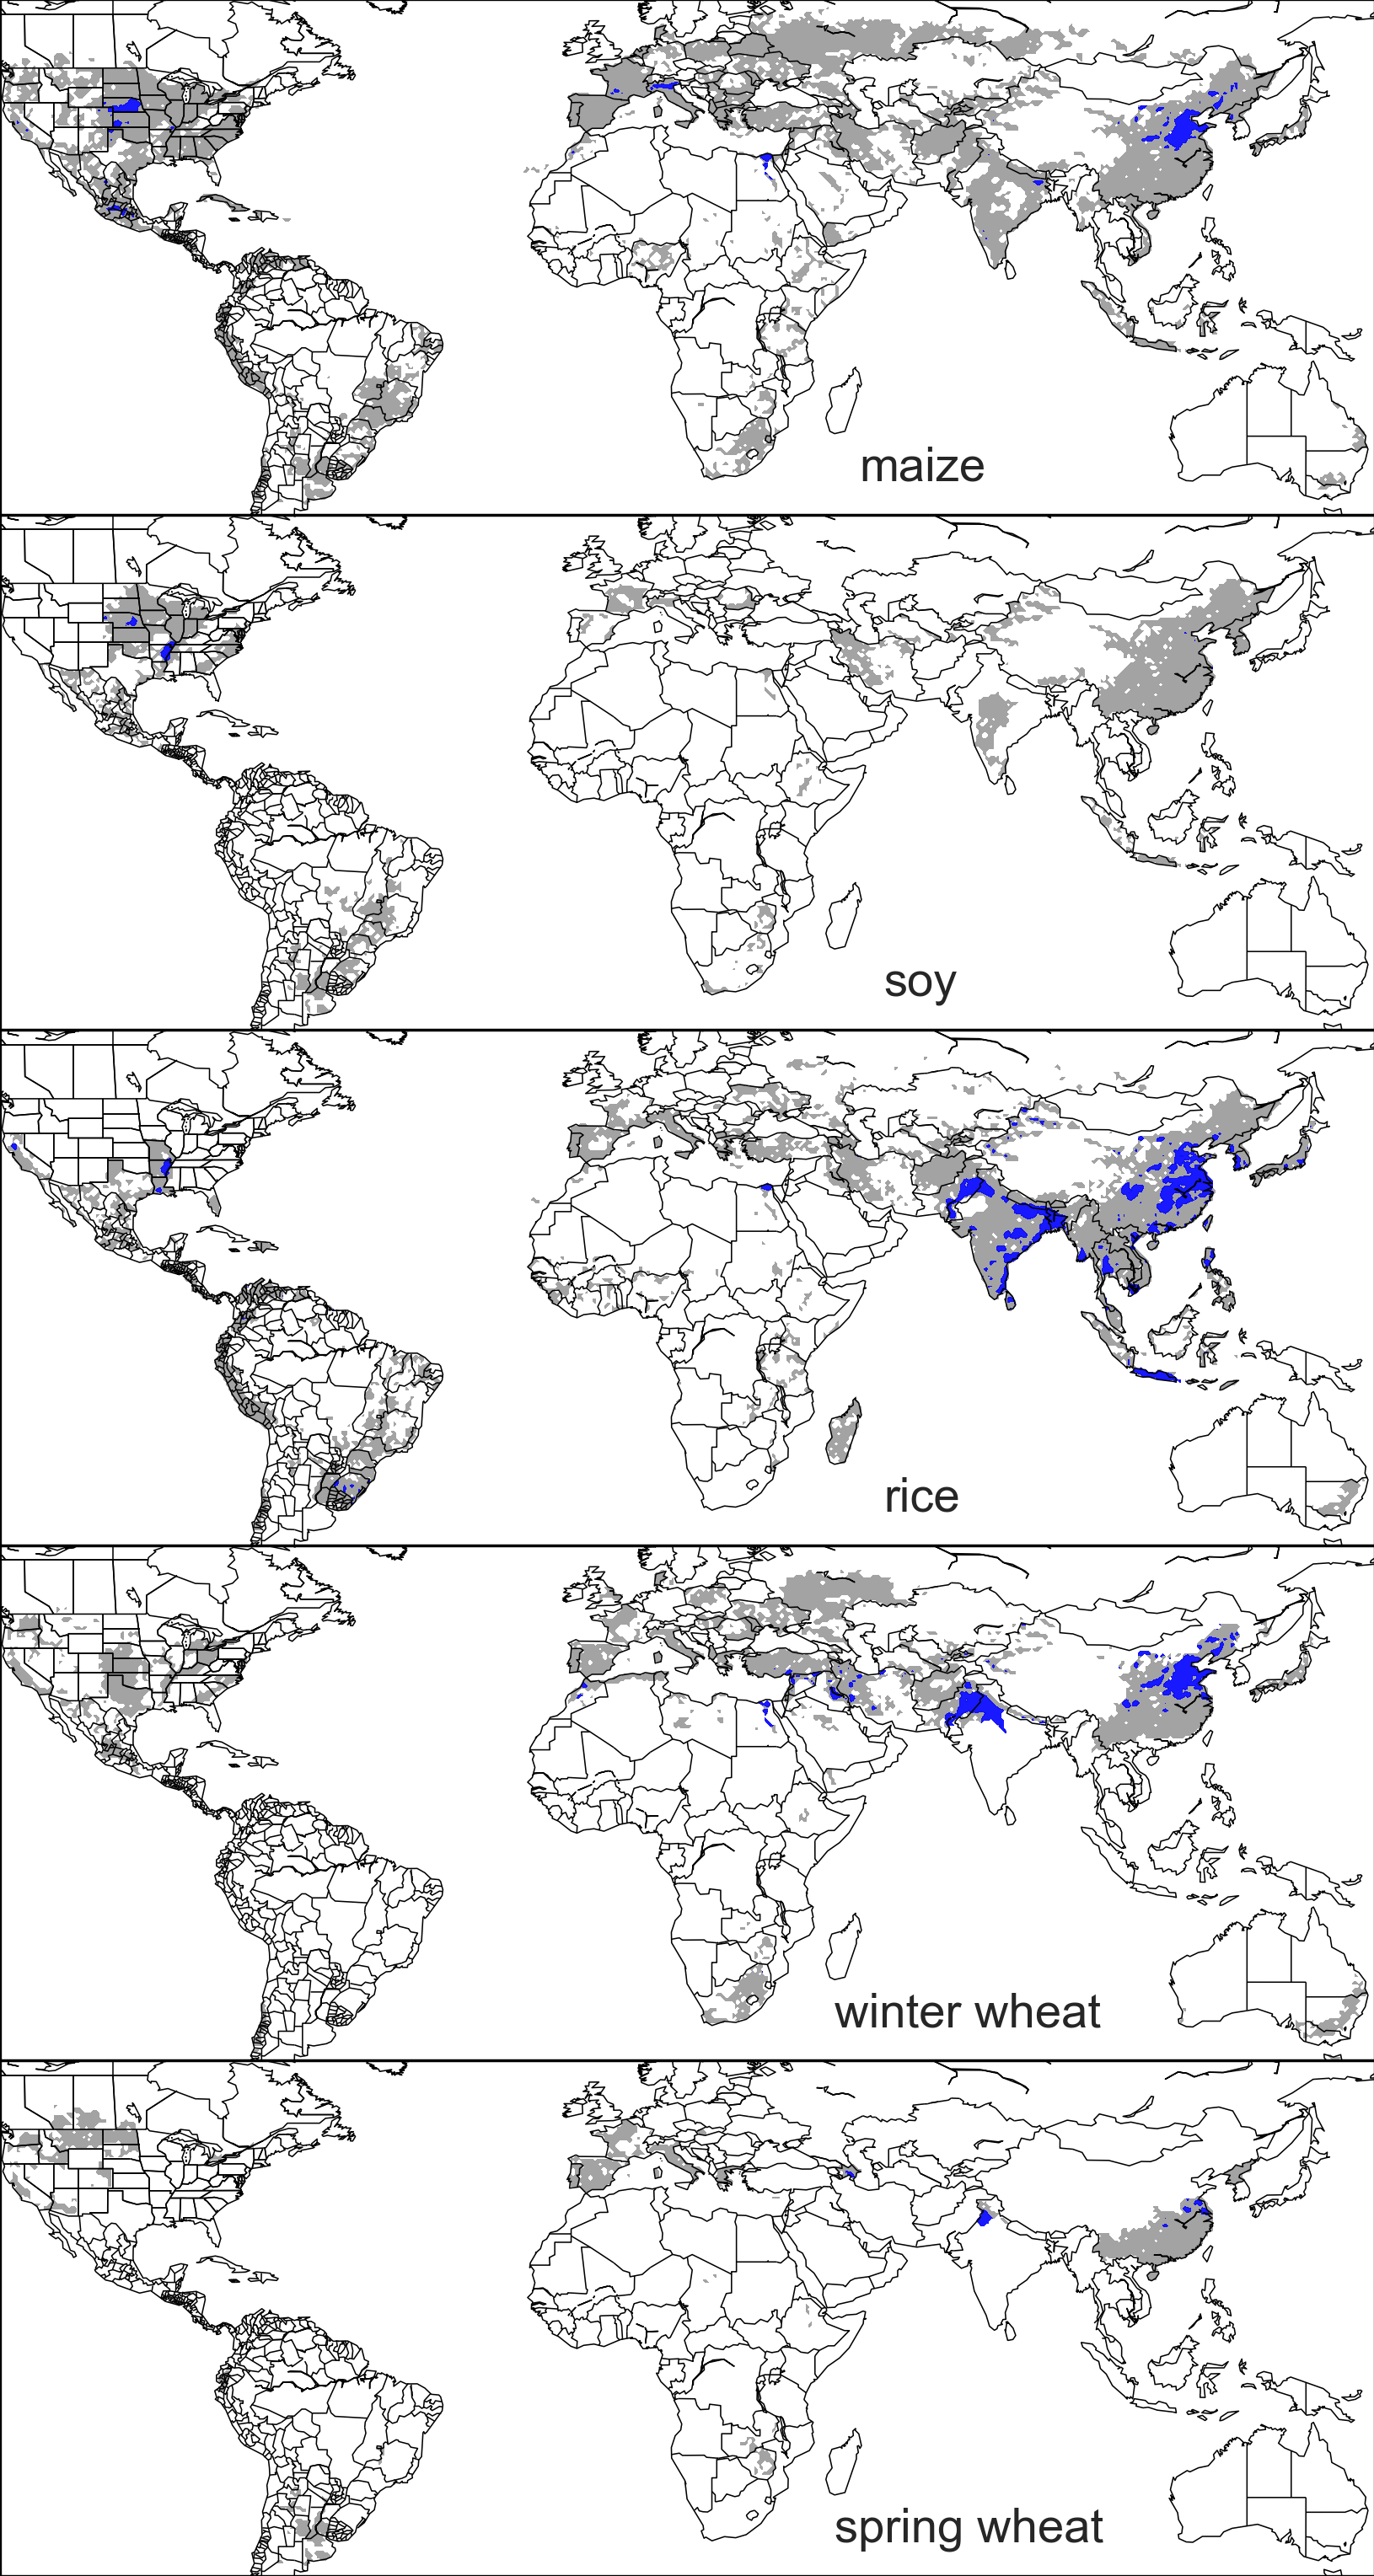
\includegraphics[width=\textwidth]{s_croparea_irr.png}\\
    \caption{Presently cultivated area for irrigated crops in the real world. The blue contour area indicates grid-cells with more that 20,00 hectares of crop cultivated. The gray contour shows area with more that 10 hectares cultivated. Data from the MIRCA2000 data set for maize, rice, and soy. Winter and spring wheat areas are adapted from MIRCA2000 data and sorted by growing season.}
    \label{fig:irrarea}
\end{minipage}
\hspace{.05\linewidth}
%S2
\begin{minipage}{.45\textwidth}
    \centering
    \vspace{-19mm}
    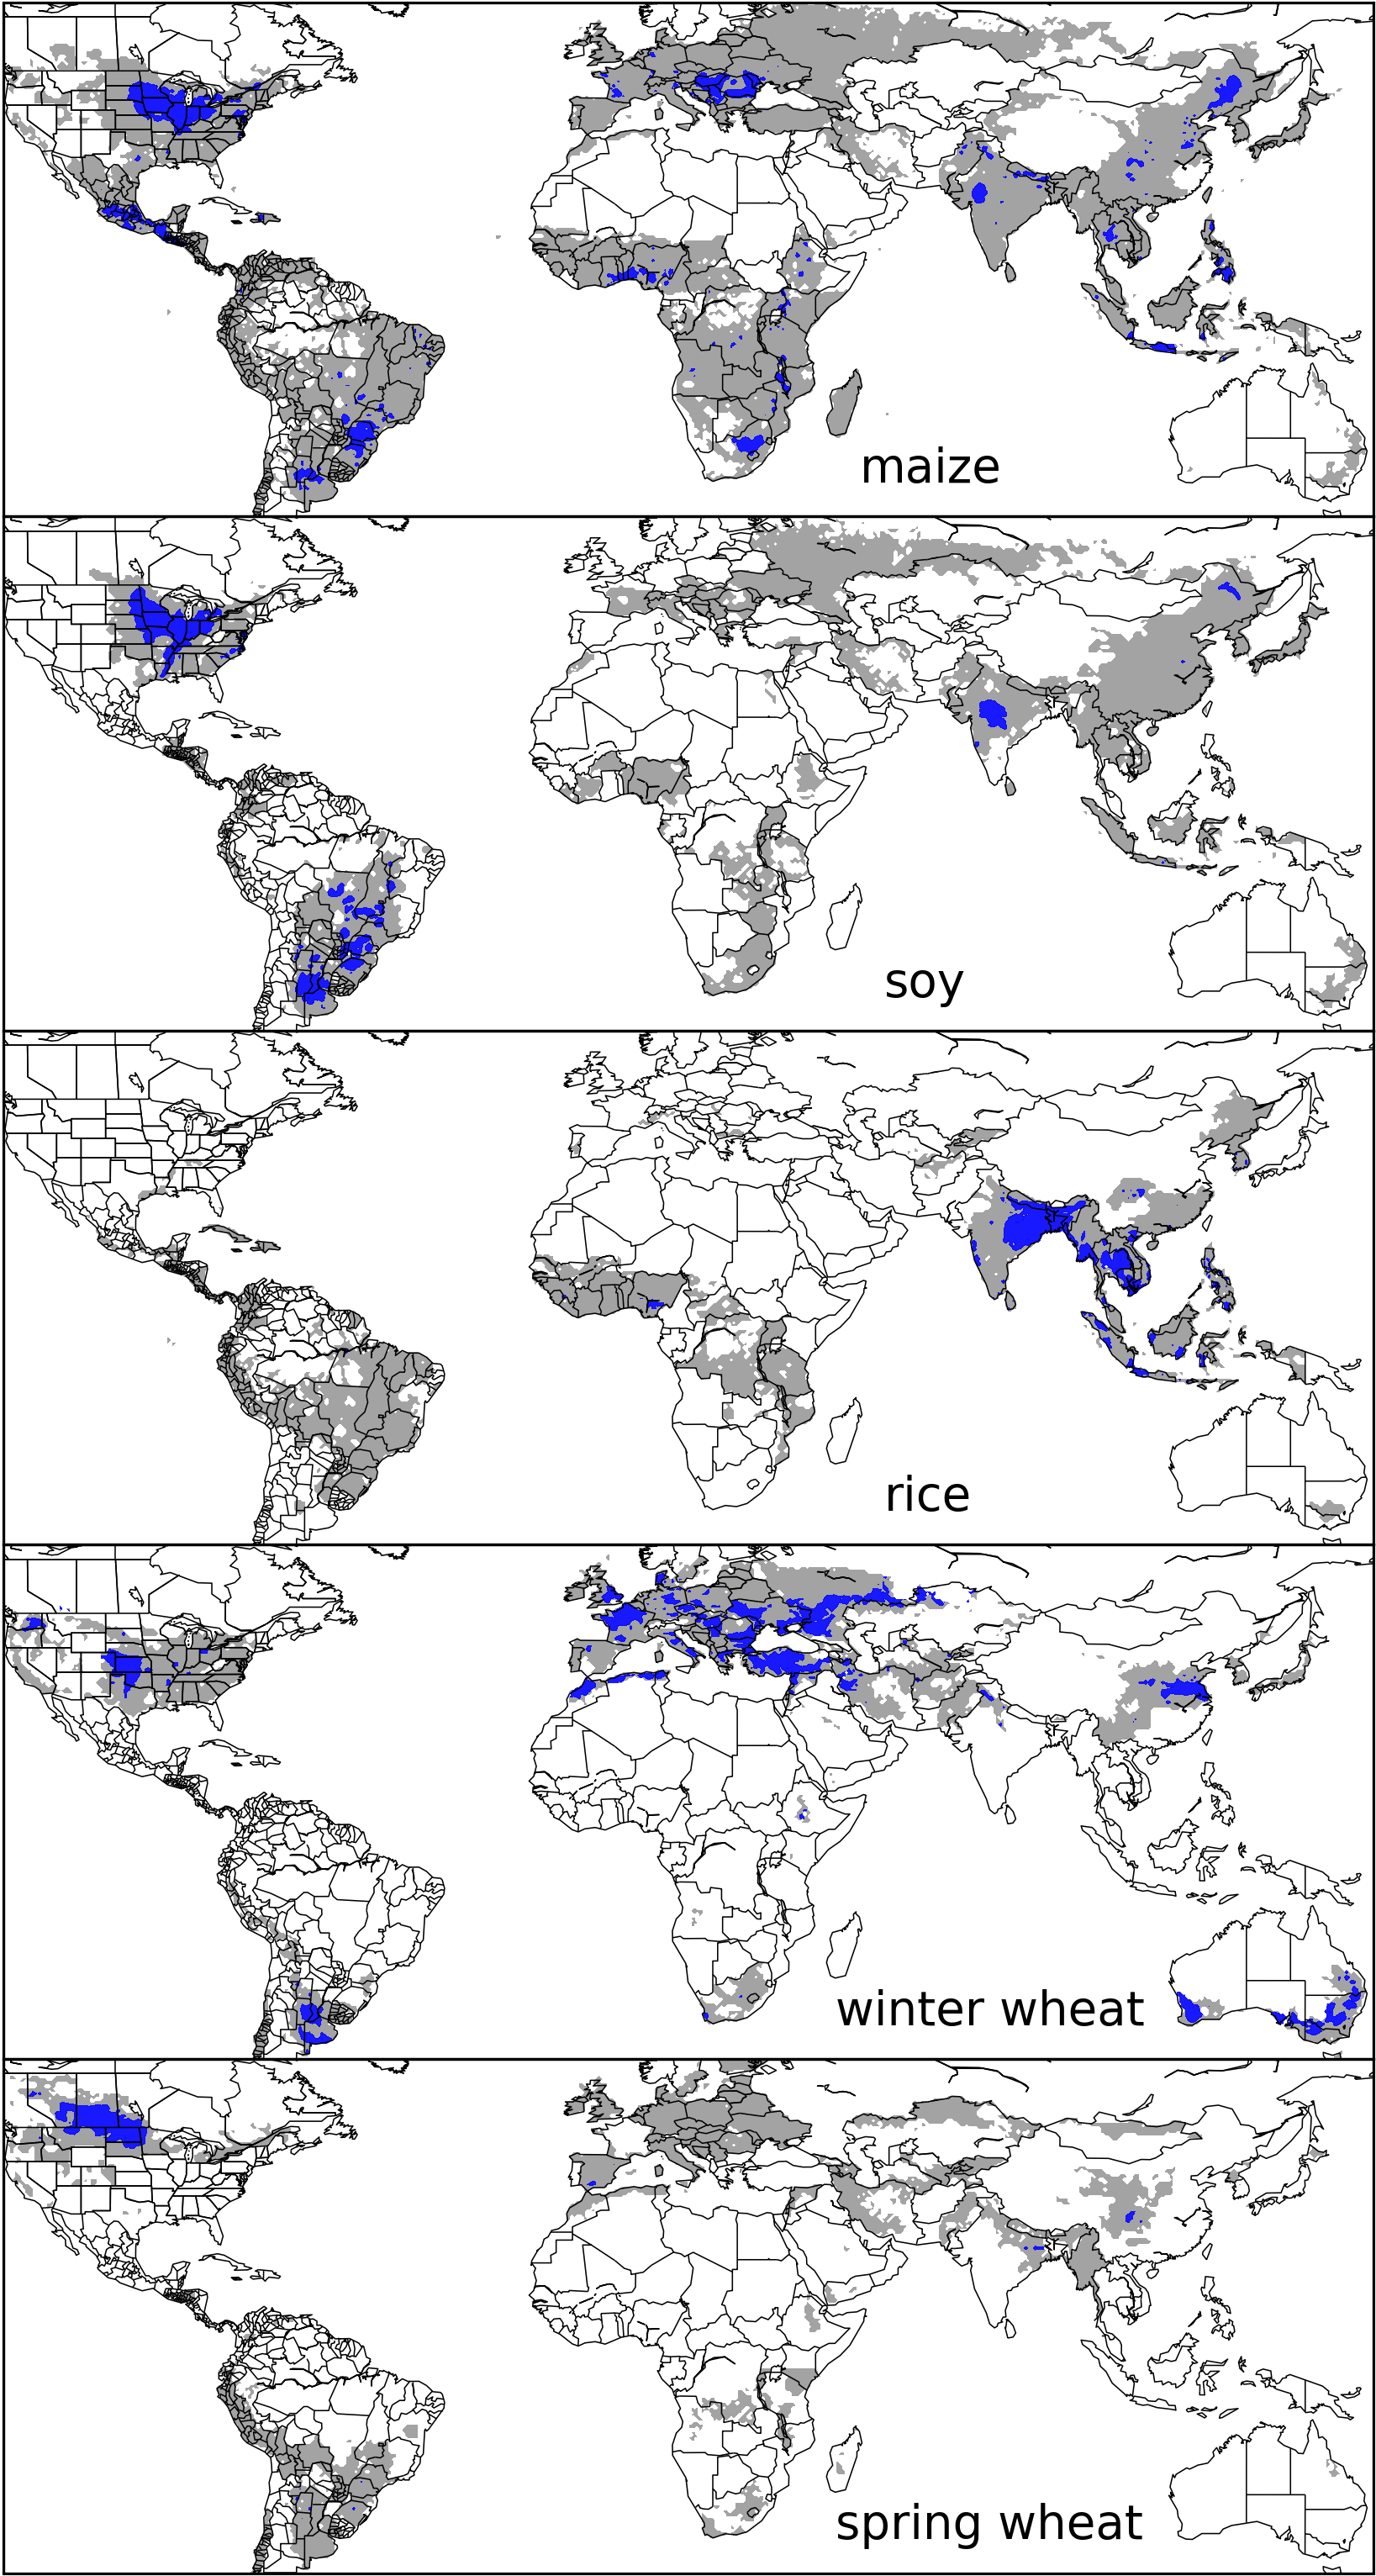
\includegraphics[width=\textwidth]{s_croparea.png}\\
    \caption{Presently cultivated area for rain fed crops in the real world. Conventions as in Figure S1. This figure repeats manuscript Figure 1 for ease of comparison.}
    \label{fig:rainfed}
\end{minipage}
\end{figure}

\clearpage
\section{Reanalysis Climate Products}
\begin{figure}[h!]
    \centering
    \includegraphics[width=\textwidth]{s_precip_rea.png}
    \caption{Comparison across the three reanalysis products used in GGCMI Phase 2. Values are aggregated across cultivation area based on the MIRCA2000 dataset.}
    \label{fig:precip_rea}
\end{figure}

\begin{figure}[h!]
    \centering
    \includegraphics[width=\textwidth]{s_temp_rea.png}
    \caption{Same as Figure S3 but for temperature.}
    \label{fig:precip_rea}
\end{figure}

\clearpage
\section{Model Details}

\vspace{-4mm}
\begin{table}[h!]
    \centering
    \caption{
        Key model details. Notes: (NA where not applicable)\\
        $\textbf{a:}$ D: daily time-step; M: monthly time-step; H: hourly time-step; WG: use monthly climate data interpolated to daily using a weather-generator\\
        $\textbf{b:}$ Ta: average temperature, Tmn: minimum temperature, Tmx: maximum temperature, cld: percentage of cloud cover, sun: fraction of sunshine hours; RH: relative humidity; WS: wind speed; Vap: vapour pressure, Rad: radiation\\
        $\textbf{c:}$ Source of soil property inputs (e.g., source of basic soil properties), plus method for manipulation to derive parameters required by the model); AWC: Available Water Capacity 141; HYD: hydraulic soil parameters; THM: thermal parameters; HWSD: Harmonized world soil database 142; STC: soil texture classification based on the USDA soil texture classification (http://ufdc.ufl.edu/IR00003107/00001); ISRIC-WISE 143; ROSETTA 144\\
        $\textbf{d:}$ Number of years for spin up (x); OM: organic matter, C: organic carbon; N: organic nitrogen; NH3: ammonia; NO3: nitrate; H2O: soil water; P: phosphorus; CR: crop residues; Tsoil: soil temperature\\
        $\textbf{e:}$ calibration of model parameters other than the ones described in the original model description\\
        $\textbf{f:}$ PHU+V: prescribed externally computed phenological heat unit requirements and vernalization (winter wheat) per crop and grid cell to meet prescribed harvest date on average (1980-2010); HI: harvest index\\
        $\textbf{g:}$ Irrigation rules: depth of soil moisture measured (cm) / lower soil moisture threshold to trigger irrigation (\%); / upper soil moisture threshold to stop irrigation (\%); / irrigation application efficiency (\%); no WS: no water stress\\
        $\textbf{h:}$ Irrigation rules: EPIC-based models: water stress in crop to trigger automatic irrigation (\%); / irrigation efficiency - runoff from irrigation water (\%); / maximum of annual irrigation volume (mm); / maximum of single irrigation volume allowed (mm); / minimum of single irrigation volume allowed (mm)\\
        $\textbf{i:}$ Remove residue or not (Yes/No)\\
        $\textbf{j:}$ ET0: LSM: land surface model, complex computation of energy and water vapor fluxes\\
    }
    \vspace{-5mm}
    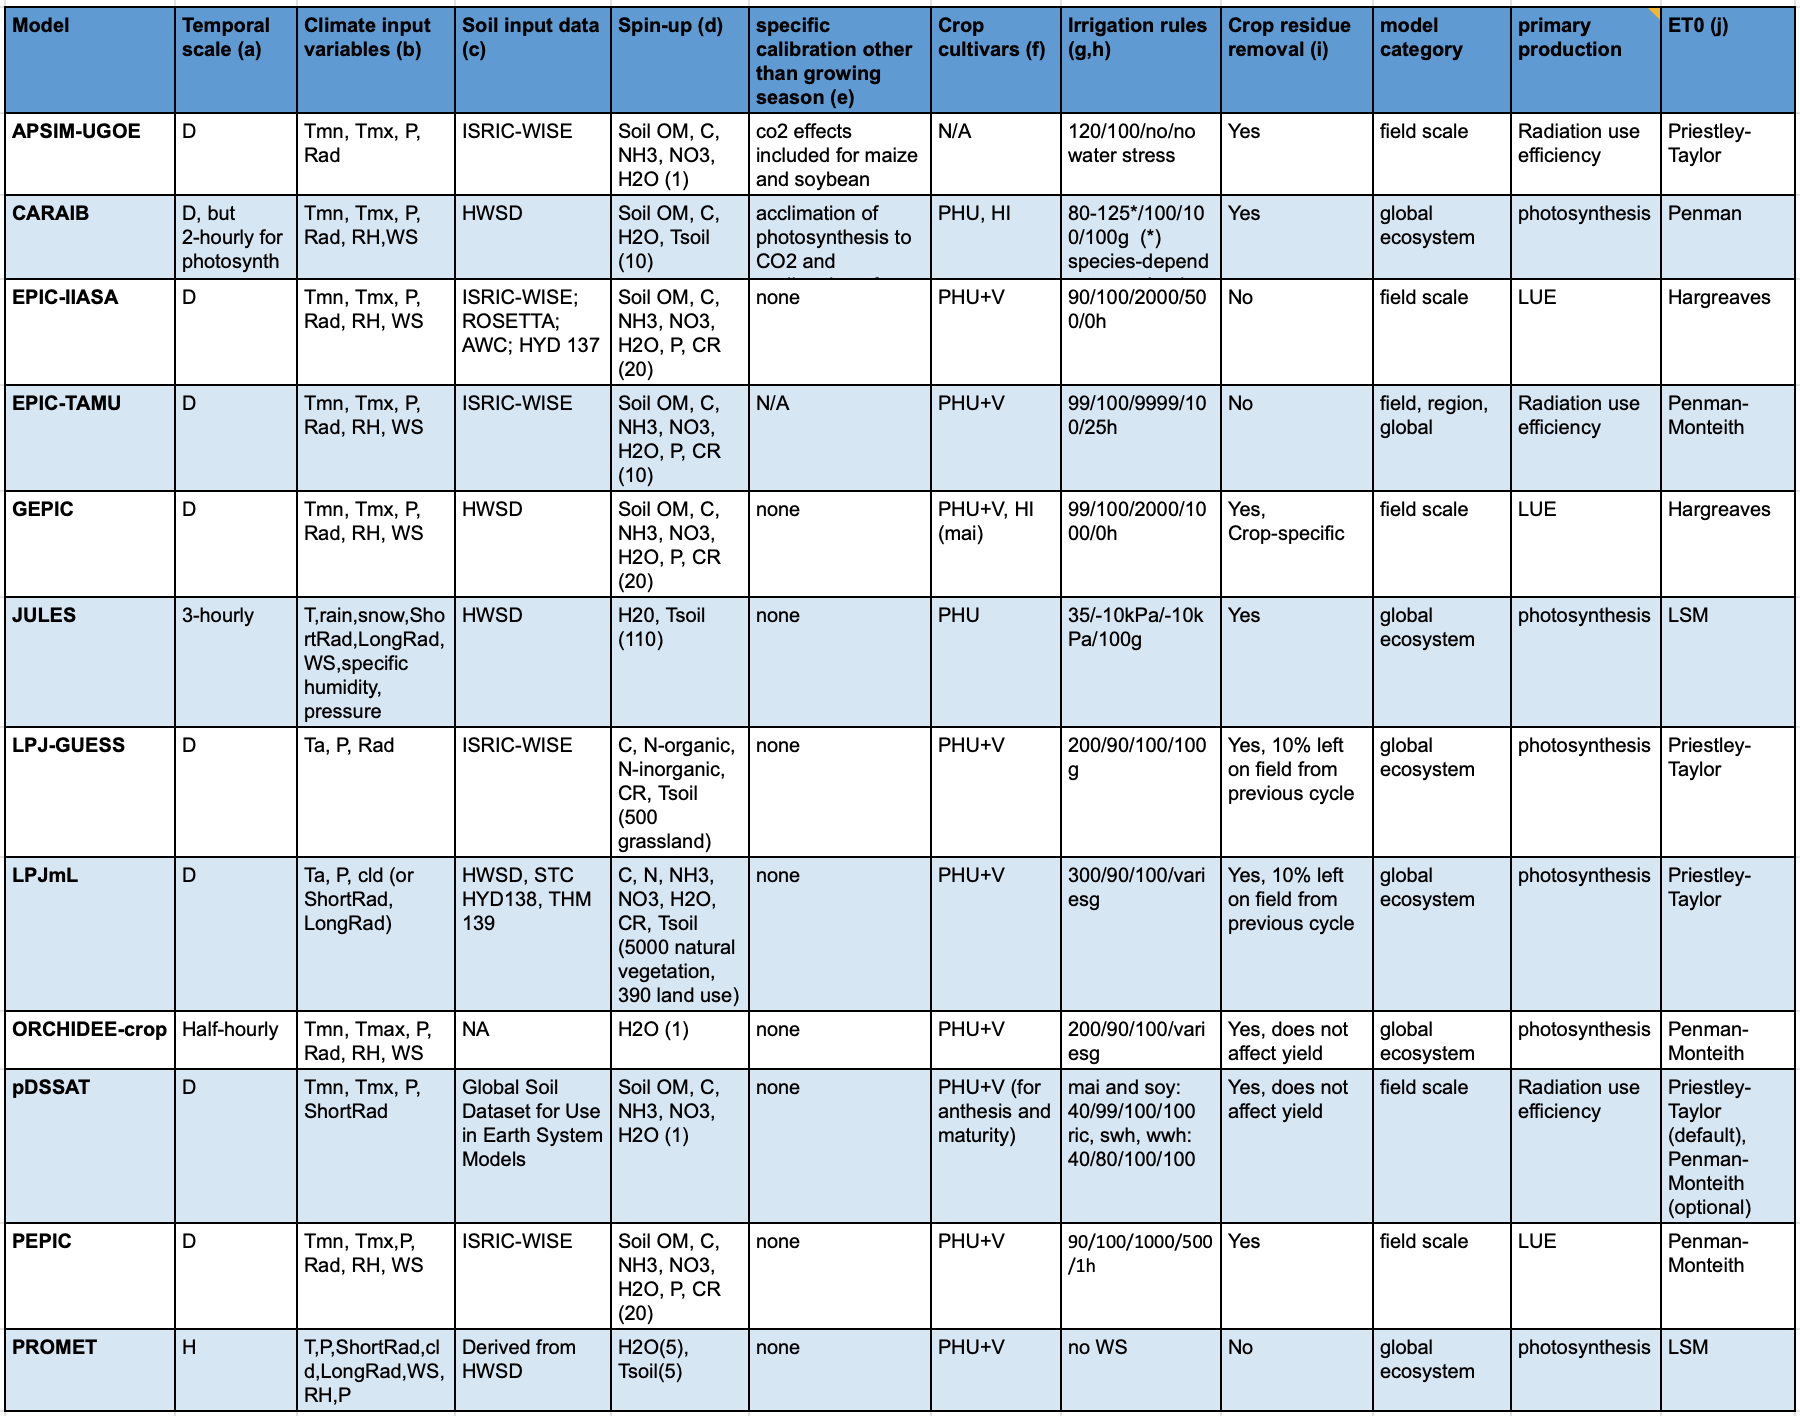
\includegraphics[width=\textwidth]{model_table.png}
    \label{fig:models}
\end{table}

Calibration procedures for growing season recalibration in the A1 scenarios:
\begin{itemize}
    \item APSIM-UGOE: default cultivars with forced harvest at given maturity days
    \item CARAIB: harvest forced on the same day as in the A0 simulation
    \item EPIC-IIASA: Potential Heat Units (PHU) were calculated for each crop and grid cell based on grid-specific input sowing and harvesting dates using the background weather dataset
    \item EPIC-TAMU: An algorithm was written to calculate the heat units required to reach maturity for a particular crop and location. These heat units were calculated for each year in the weather record, and PHU was set as the average heat units from this time series.
    \item GEPIC: Crop- and pixel-specific potential heat units (PHU) were estimated ex ante based on input sowing dates, harvest dates, and 31 year monthly means of minimum and maximum temperatures using a program provided by the EPIC development team. The resulting long-term average PHU were subsequently used as a model input parameter.
    \item JULES: Thermal times from emergence to flowering and flowering to harvest, were created by iteratively working out which thermal times would produce the right harvest dates for each crop in each gridbox (using the sowing and maturity dates provided by GGCMI and calculating harvest dates using table 11 in the Phase 1 protocol) using a 3hrly WFDEI climatology for the years 1991-2000 inclusive. The thermal time between emergence and flowering was assumed to be a crop-specific constant fraction of the thermal time between emergence and harvest. These thermal times were then prescribed as crop- and grid-cell specific values.
    \item LPJ-GUESS: In a preparatory simulation run with unlimited growing season length, the accumulated phenological heat units (PHU) at the given maturity date were recorded per crop, year and grid cell. These heat units were averaged over all years and then prescribed as crop- and grid-cell specific values.
    \item LPJmL: In a preparatory simulation run with unlimited growing season length, the accumulated phenological heat units (PHU) at the given maturity date were recorded per crop, year and grid cell. These heat units were averaged over all years and then prescribed as crop- and grid-cell specific values.
    \item ORCHIDEE-crop: Crop-specific thermal times from emergence to flowering and flowering to harvest were created from default datasets of cultivars, by a testing simulation during 2000s, we chose the cultivar best matching the  calendar provided by the protocol.
    \item pDSSAT: ran a calibration simulation in the baseline period, proportionally adjusting the phenological GDD parameters (p1 and p5 for grains) to produce thr target average growing season length over the baseline period. The resulting calibrated parameters were used for future simulations. 
    \item PEPIC: used averaged month temperature across the study period, prescribed growing season, and crop-specific base temperature to estimate PHU for each grid and crop
    \item PROMET: In a preparatory sensitivity analysis, simulation runs with unlimited growing season length were carried out for different cultivars. A 'cultivar factor' was set to a crop, year and grid cell specific value that reproduces the statistical growing season. This 'cultivar factor'  was averaged over all 30 years and then prescribed as crop- and grid-cell specific values.
\end{itemize}

\clearpage
\section{Results}

\begin{figure}[h!]
    \centering
    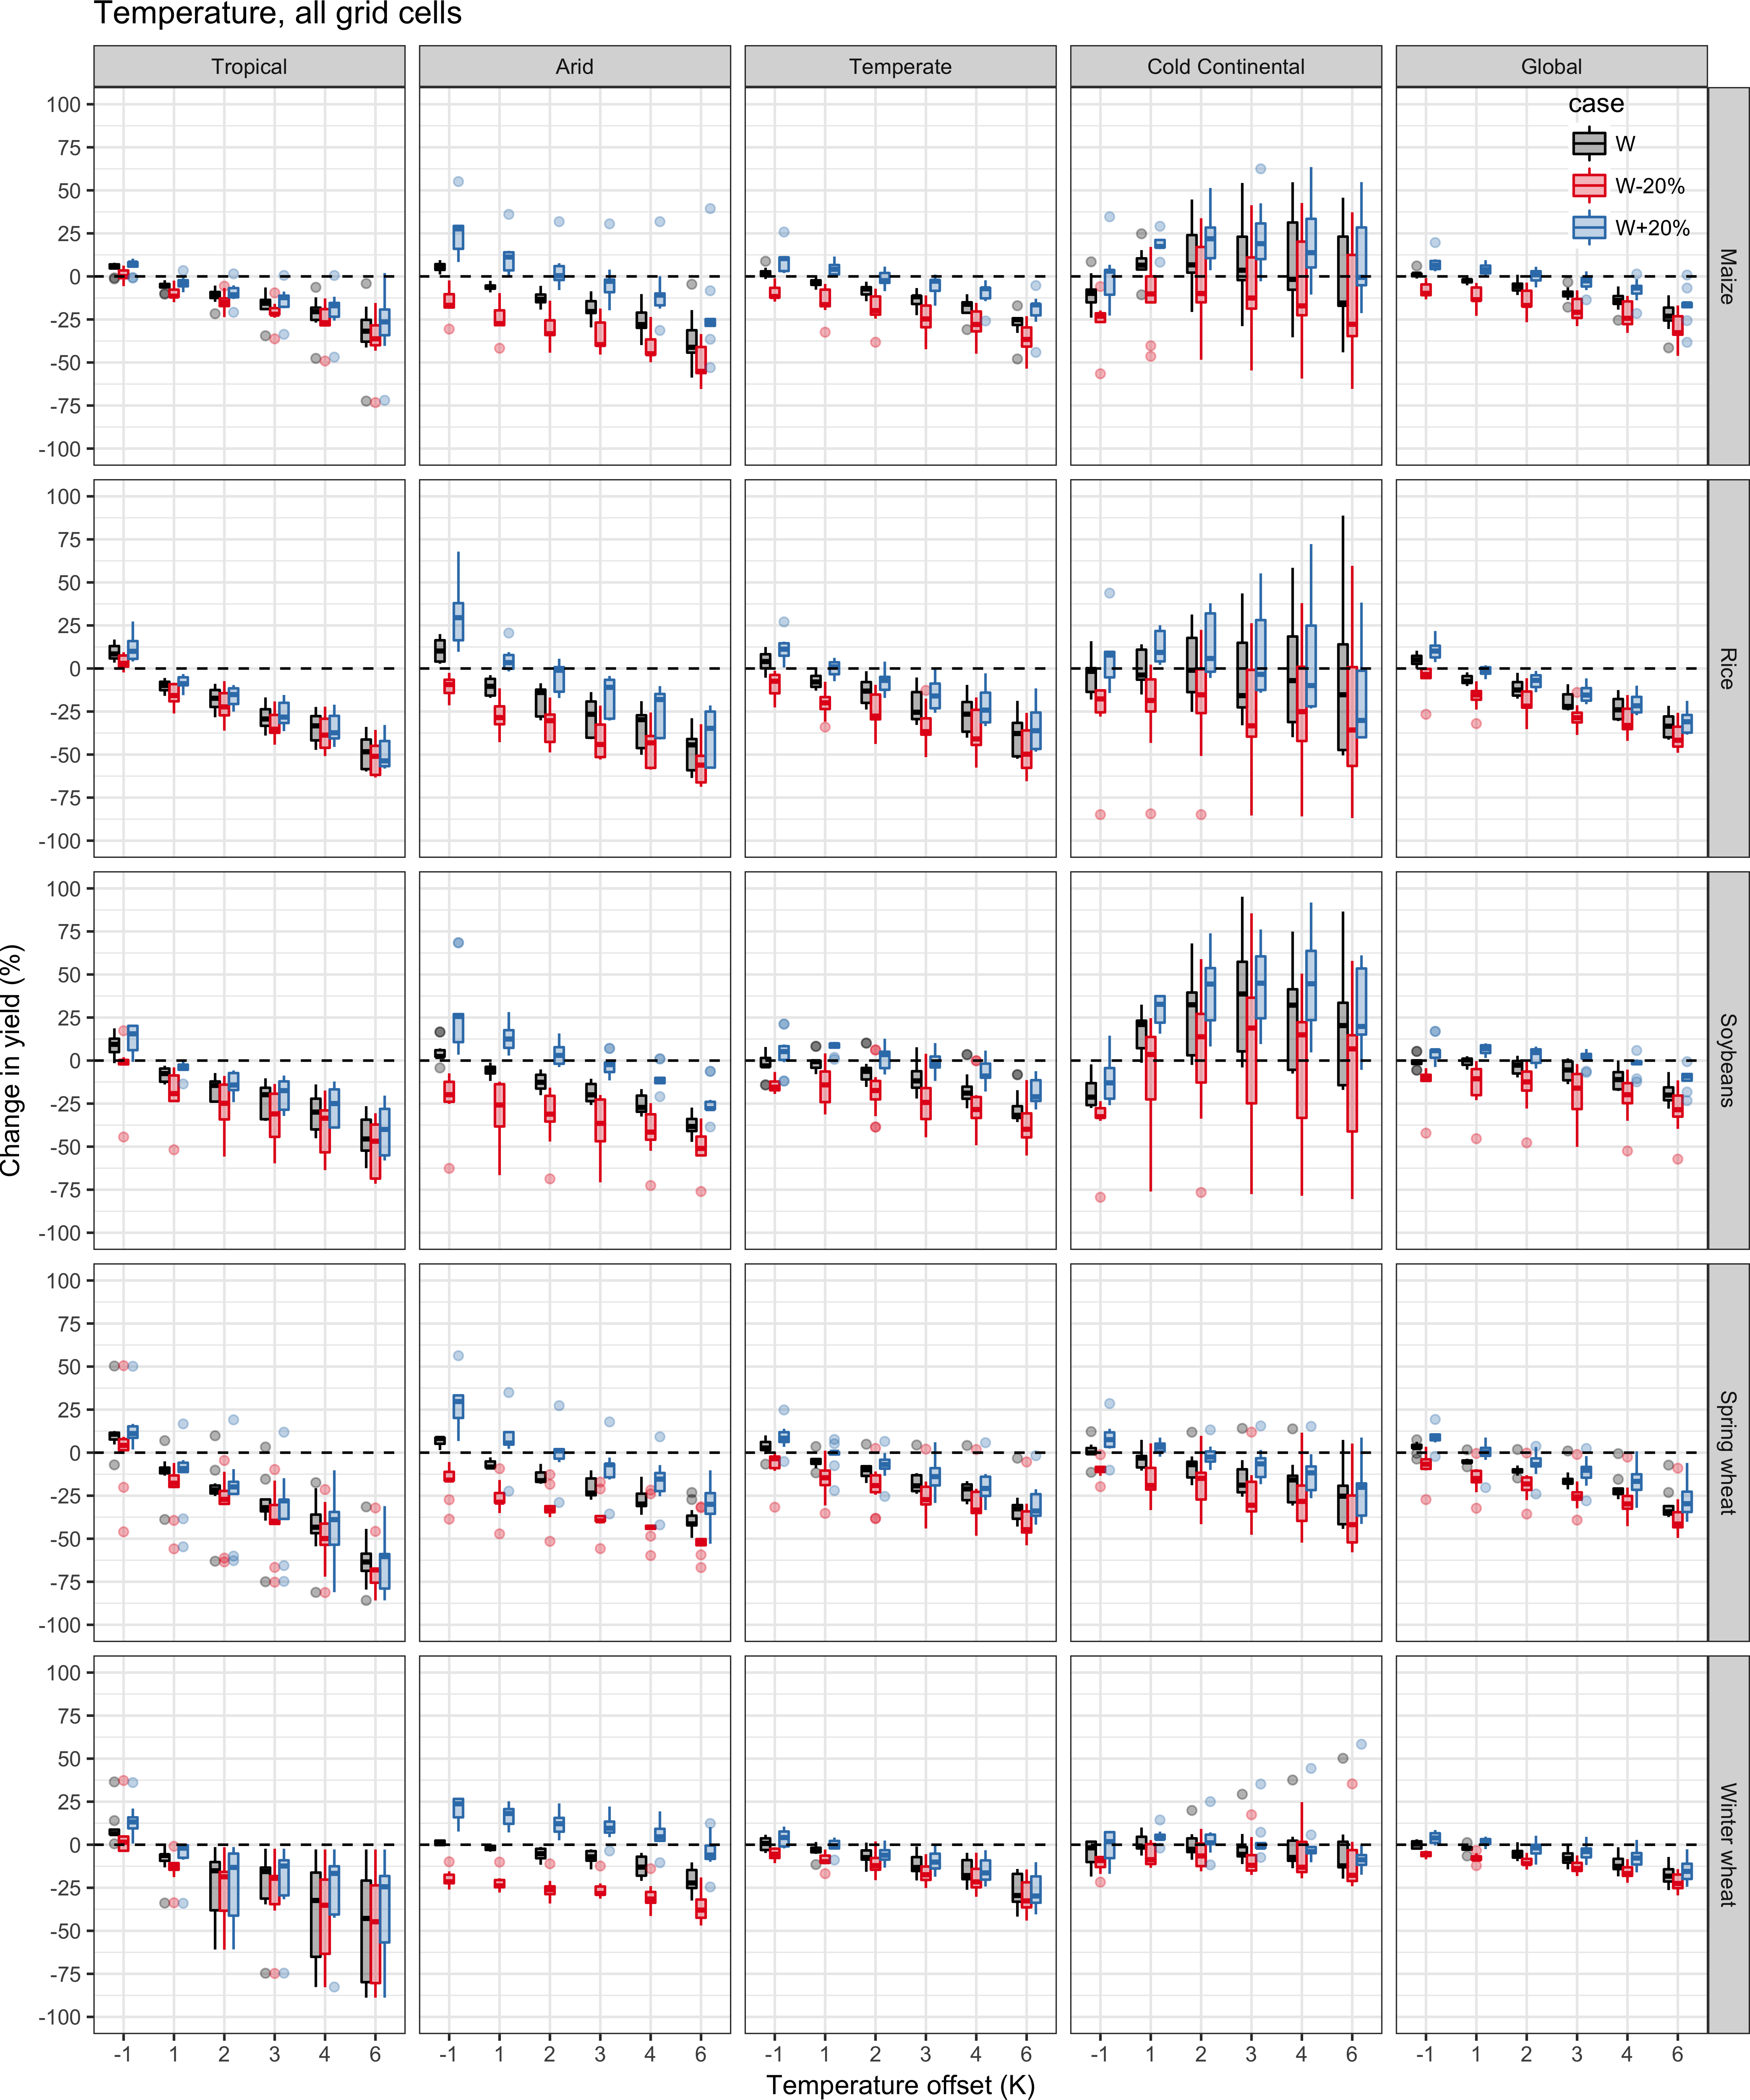
\includegraphics[width=\textwidth]{s_sim_CG_T.png}
    \caption{Same as main Figure 5a for all crops.}
    \label{fig:temperautre}
\end{figure}

\begin{figure}[h!]
    \centering
    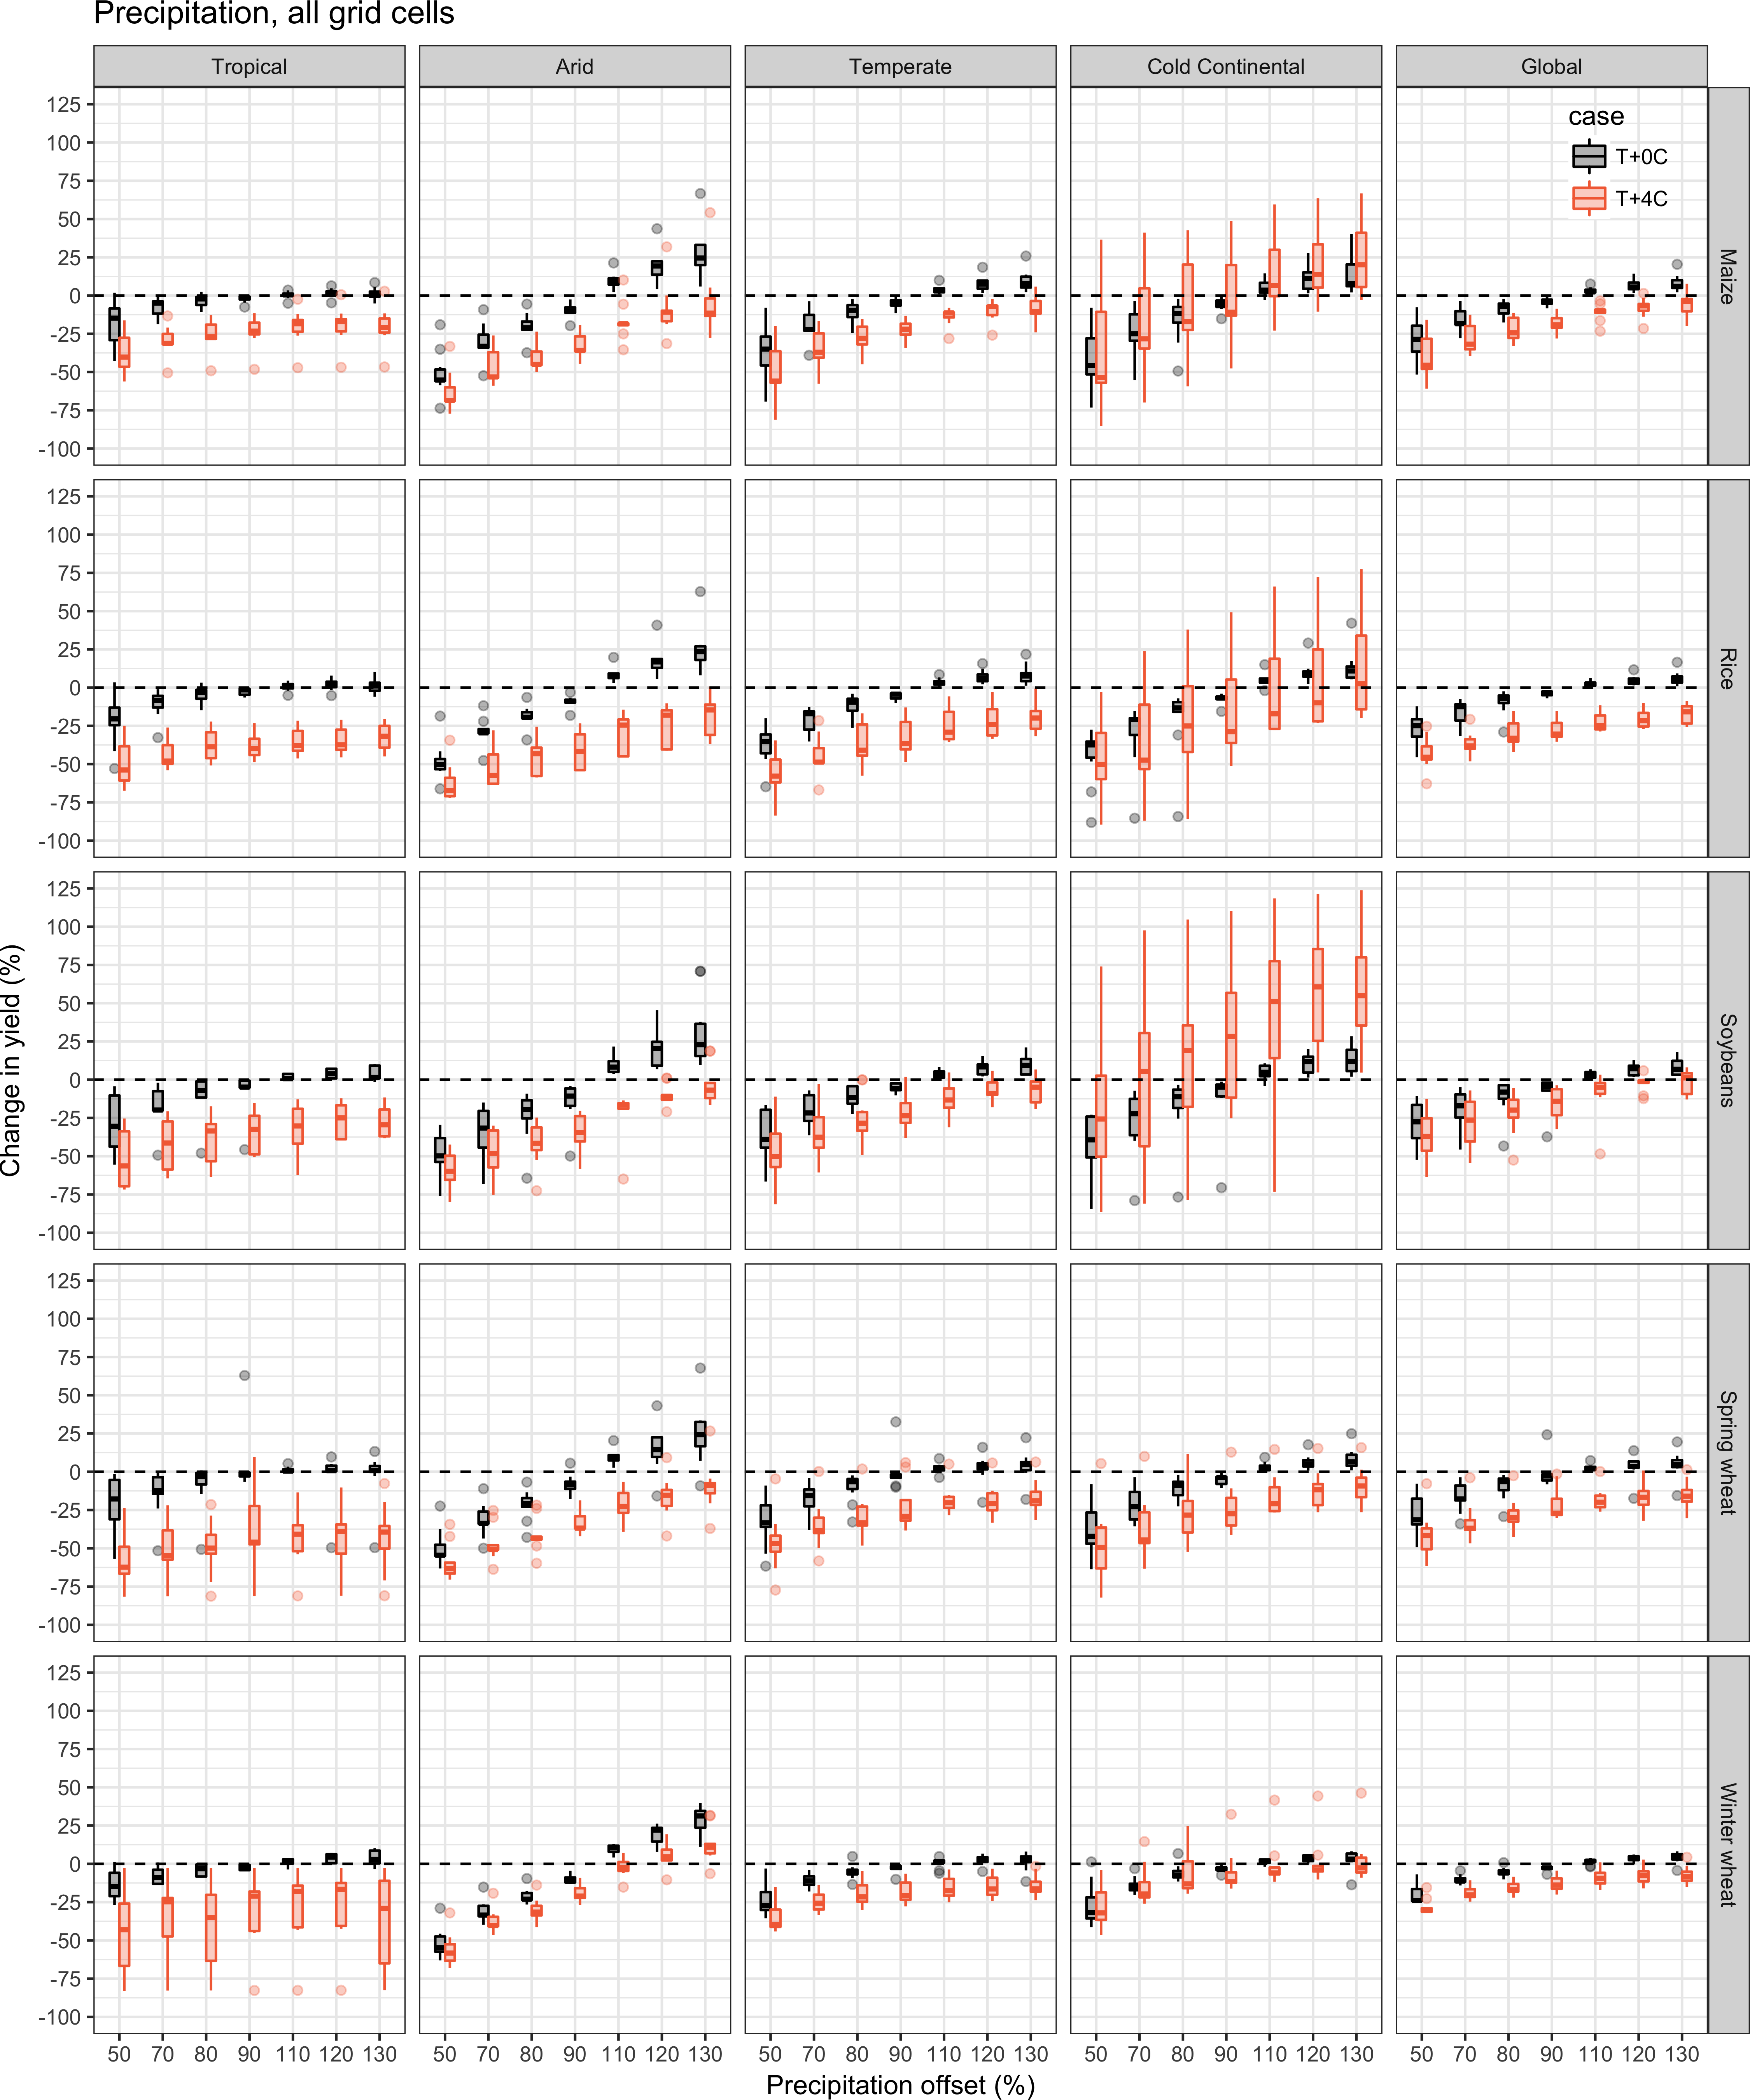
\includegraphics[width=\textwidth]{s_sim_CG_W.png}
    \caption{Same as main Figure 5b for all crops.}
    \label{fig:water}
\end{figure}

\begin{figure}[h!]
    \centering
    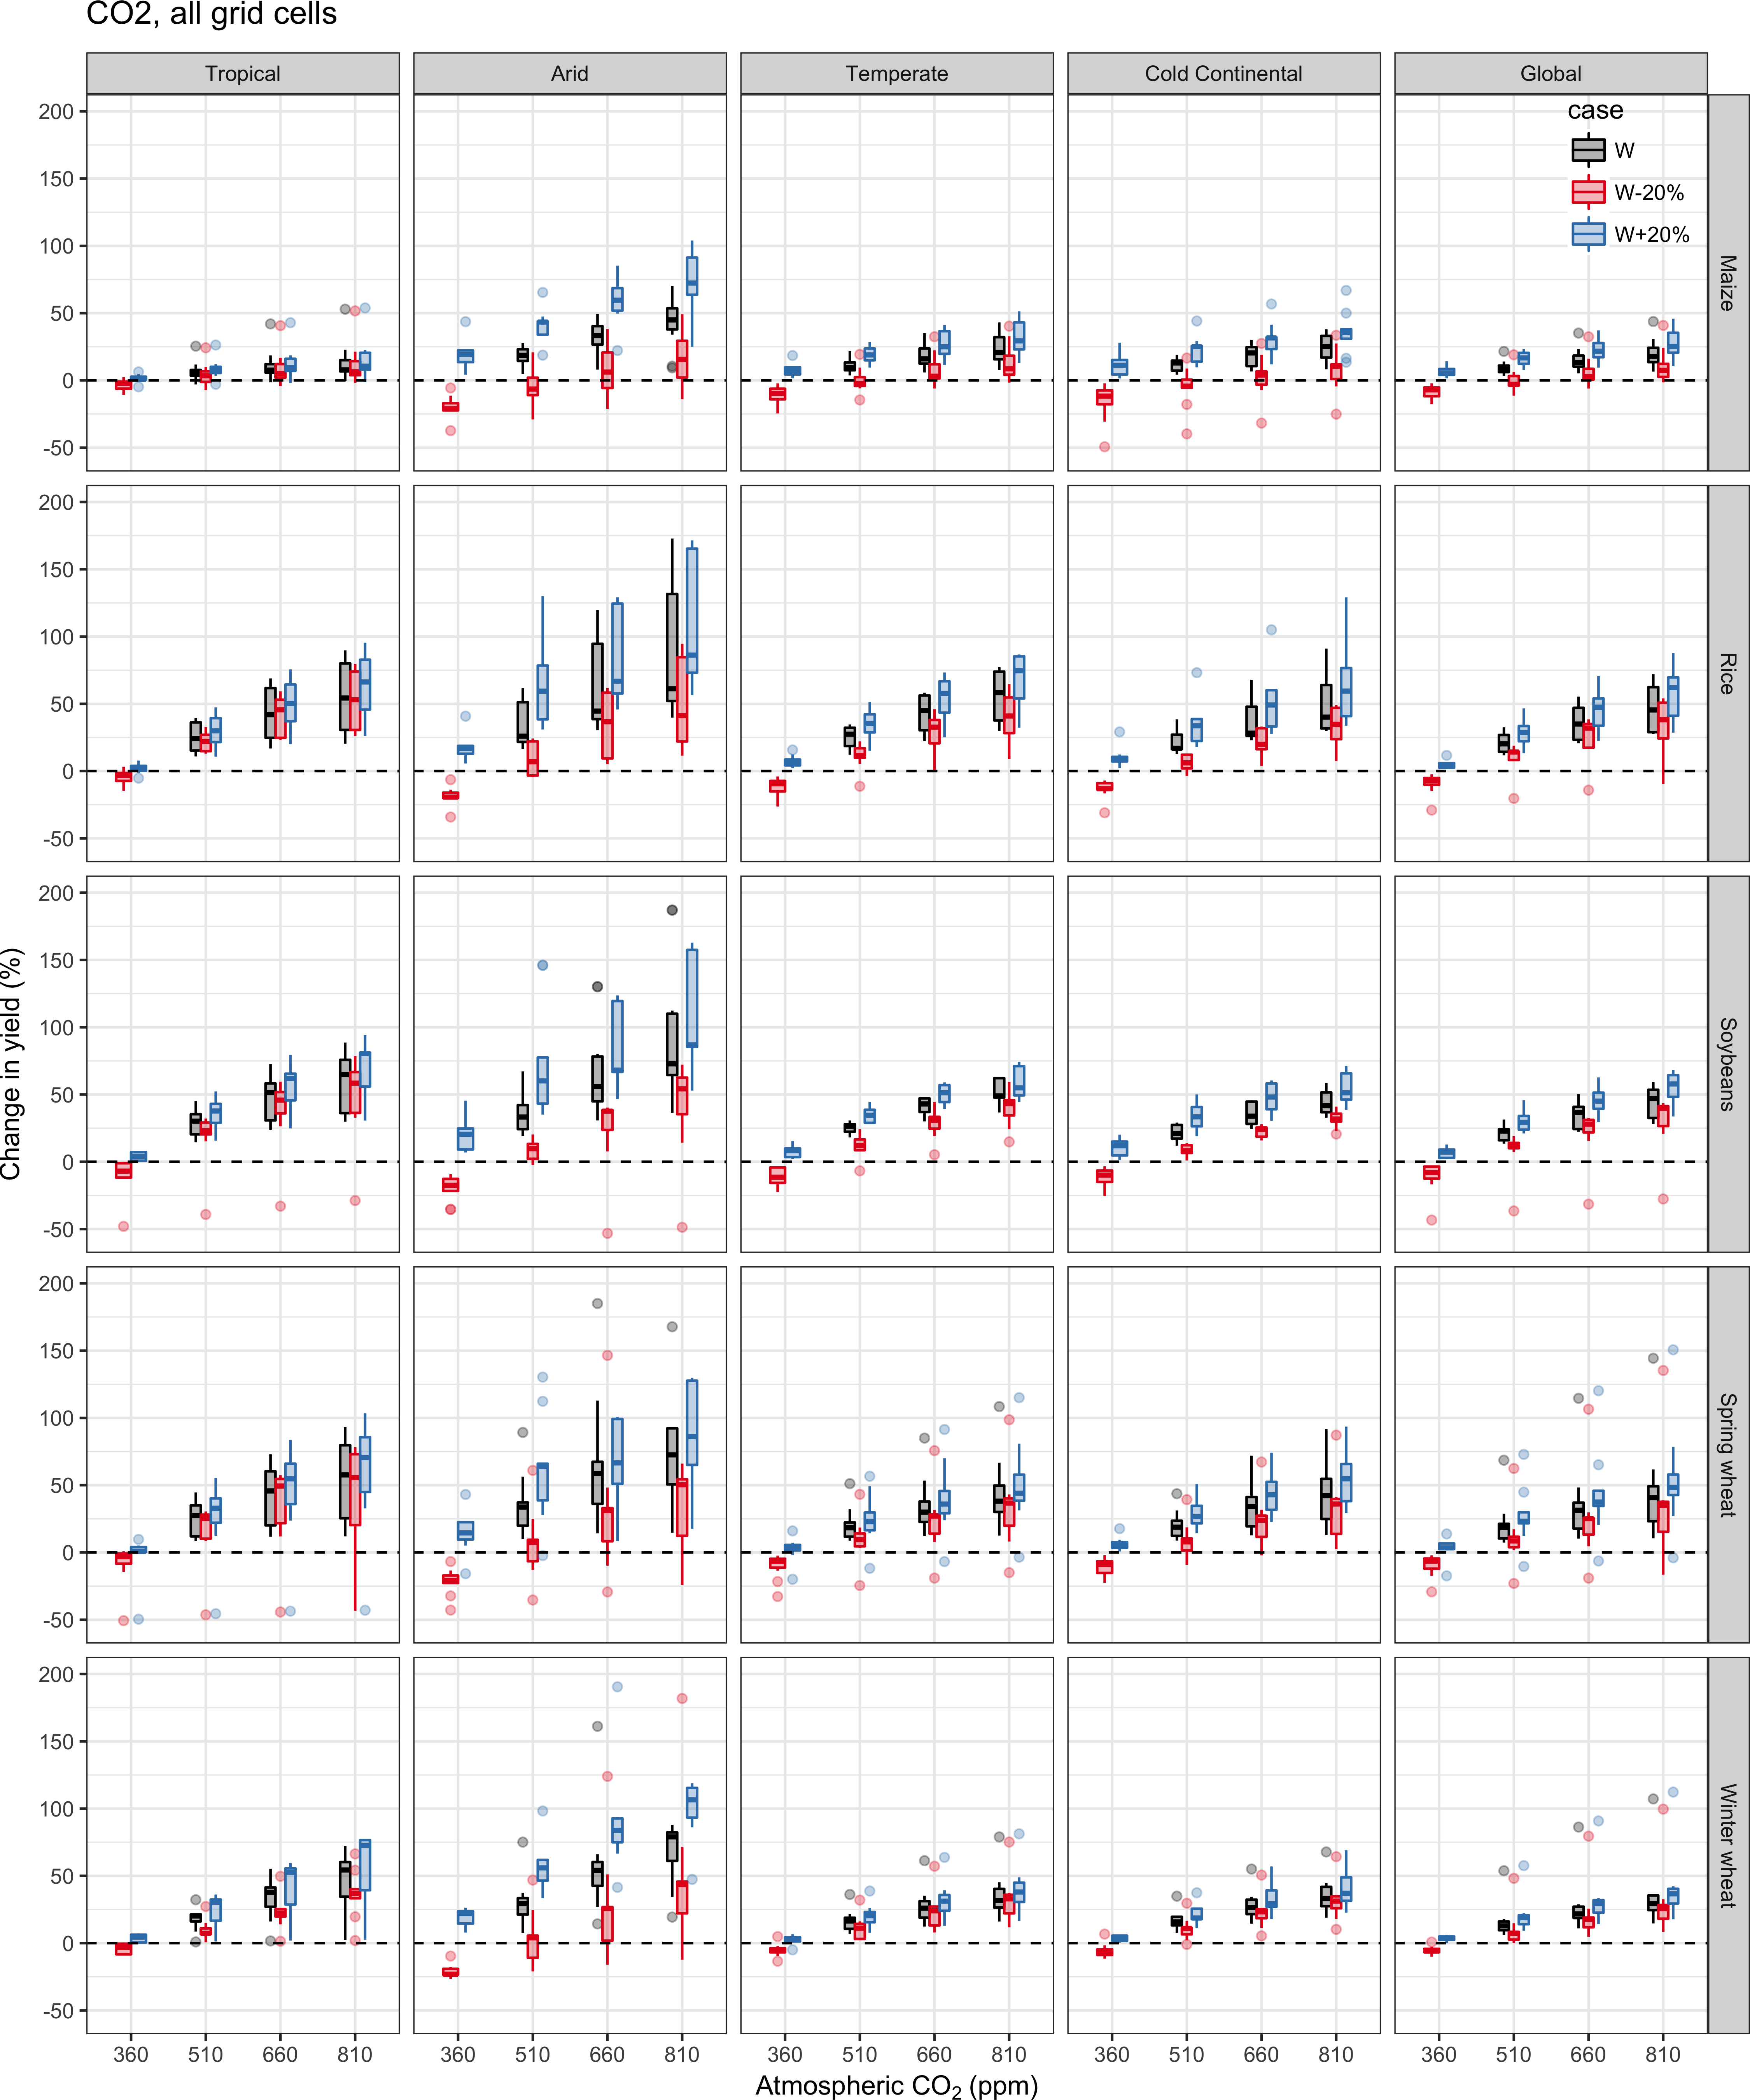
\includegraphics[width=\textwidth]{s_sim_CG_C.png}
    \caption{Same as main Figure 6a for all crops.}
    \label{fig:carbon}
\end{figure}

\begin{figure}[h!]
    \centering
    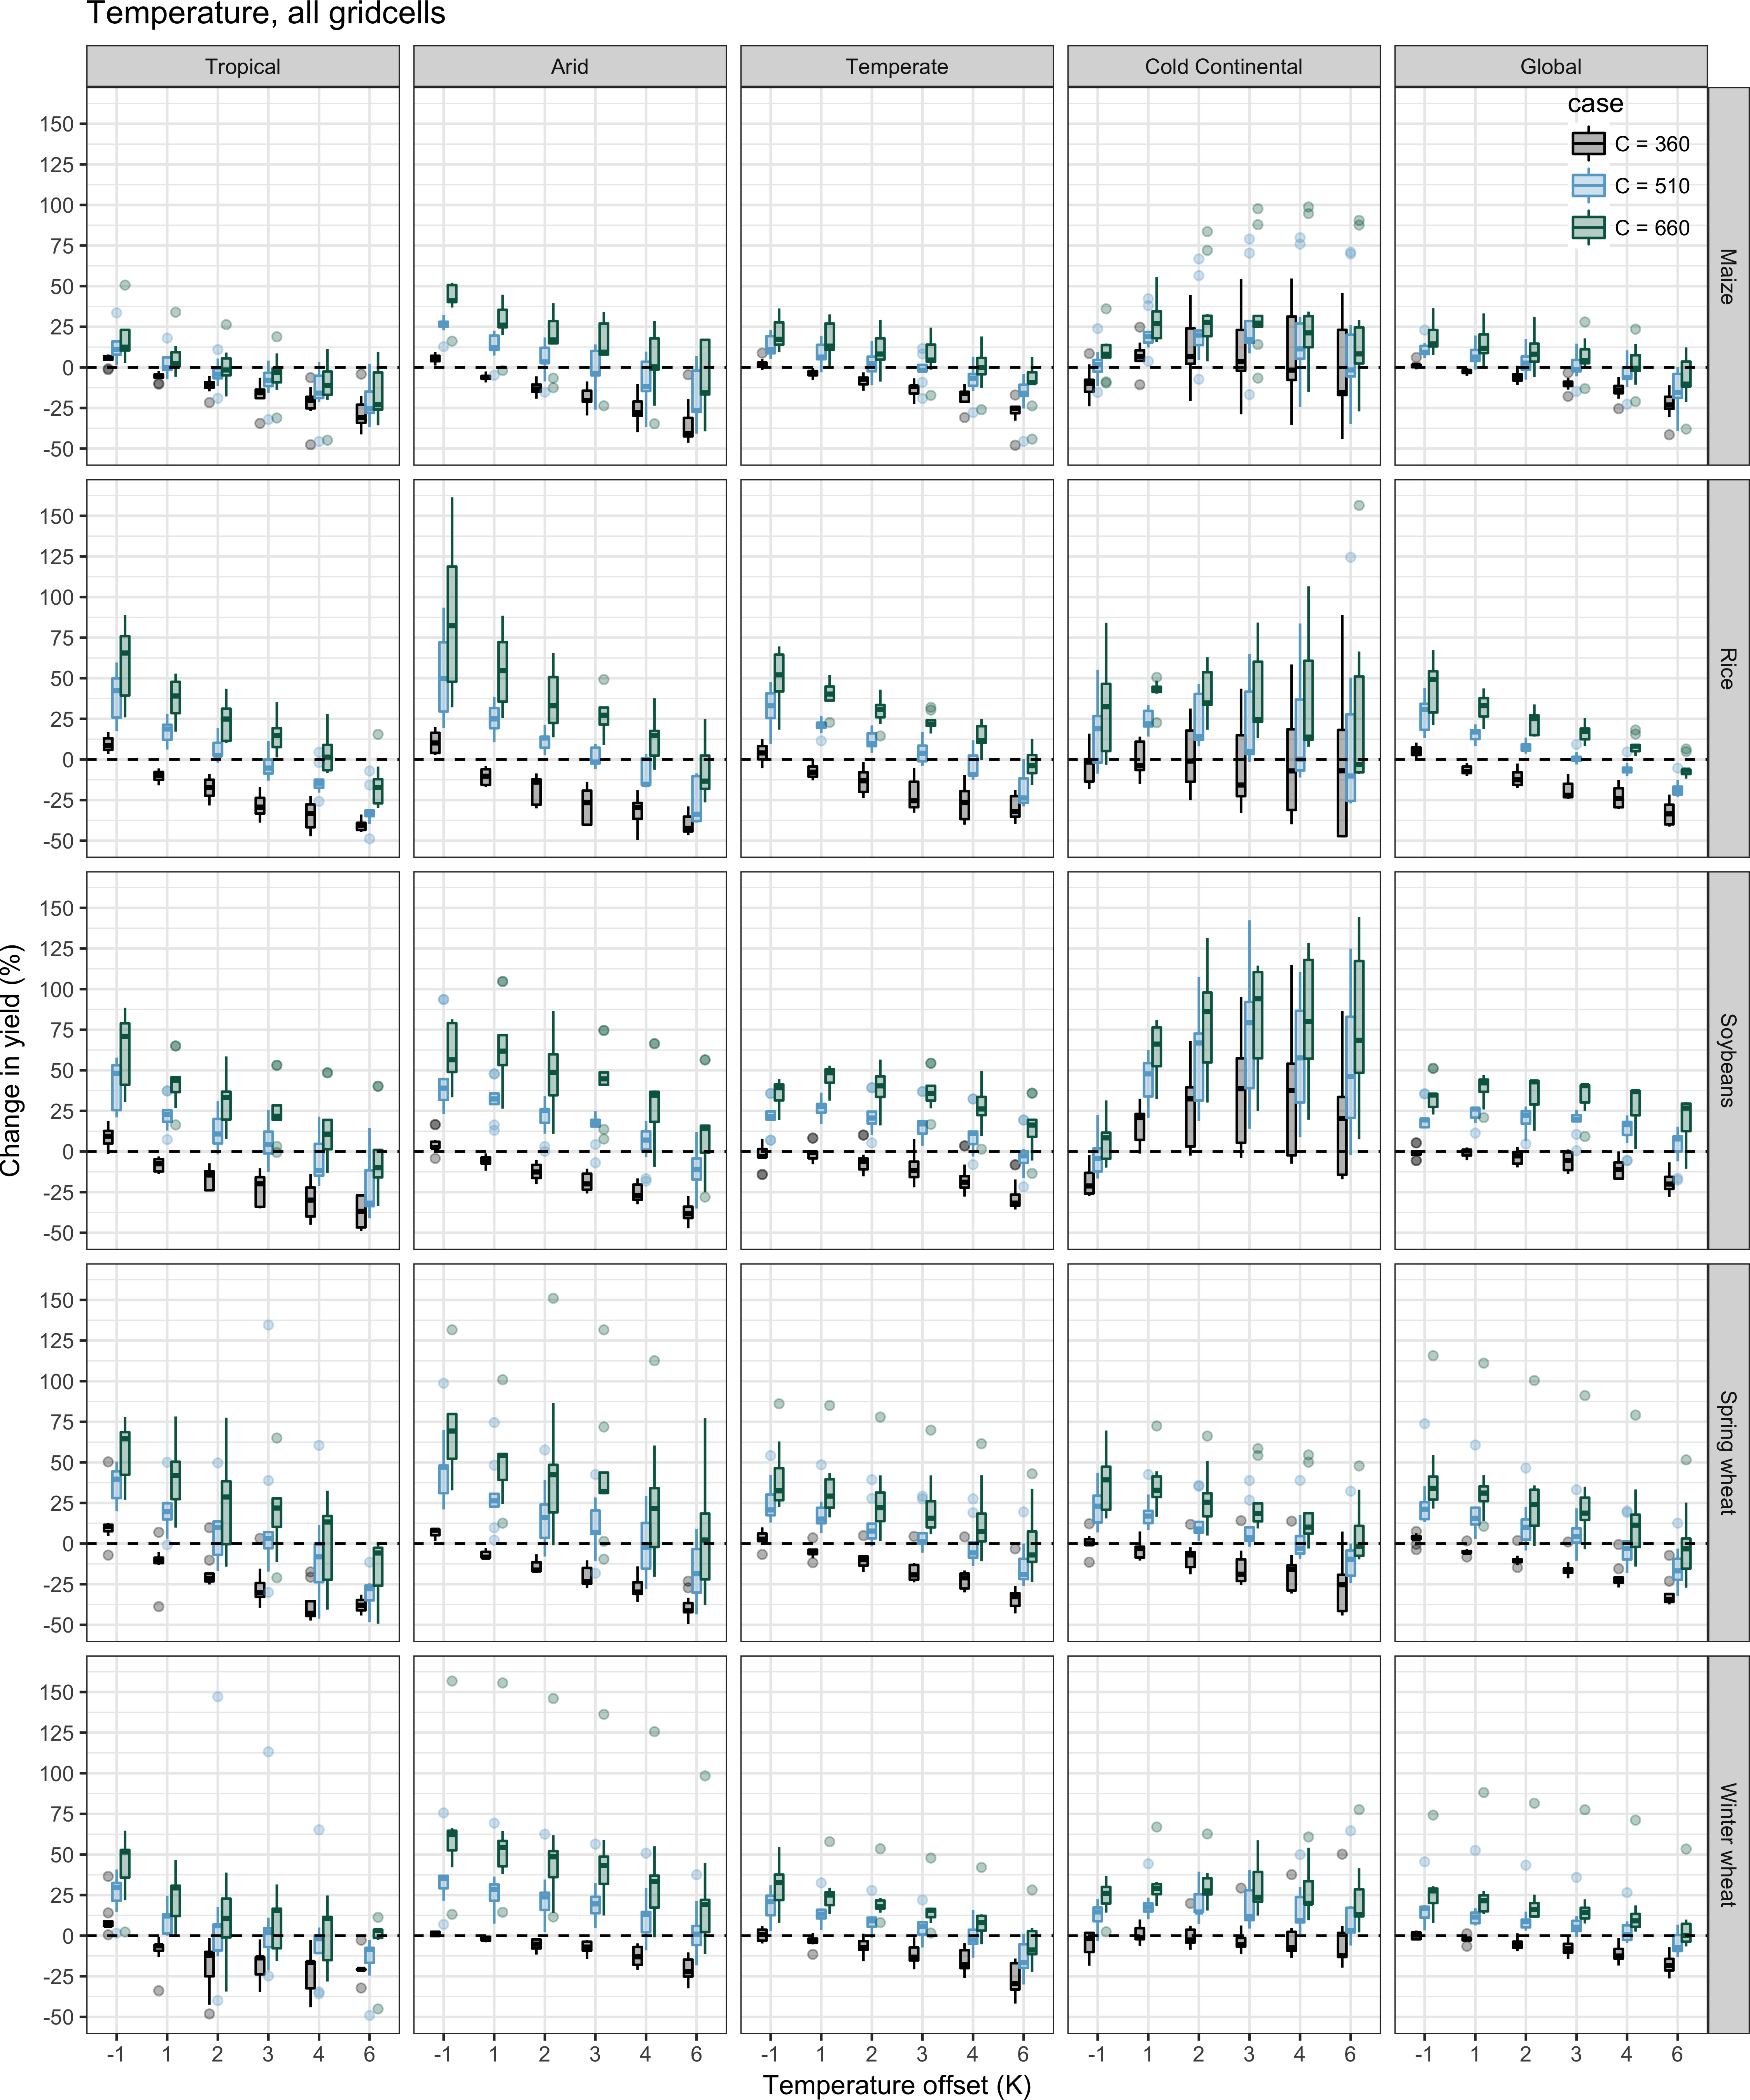
\includegraphics[width=\textwidth]{s_sim_CG_TC.png}
    \caption{Same as main Figure 6b for all crops.}
    \label{fig:carbontemp}
\end{figure}

\begin{figure}[h!]
    \centering
    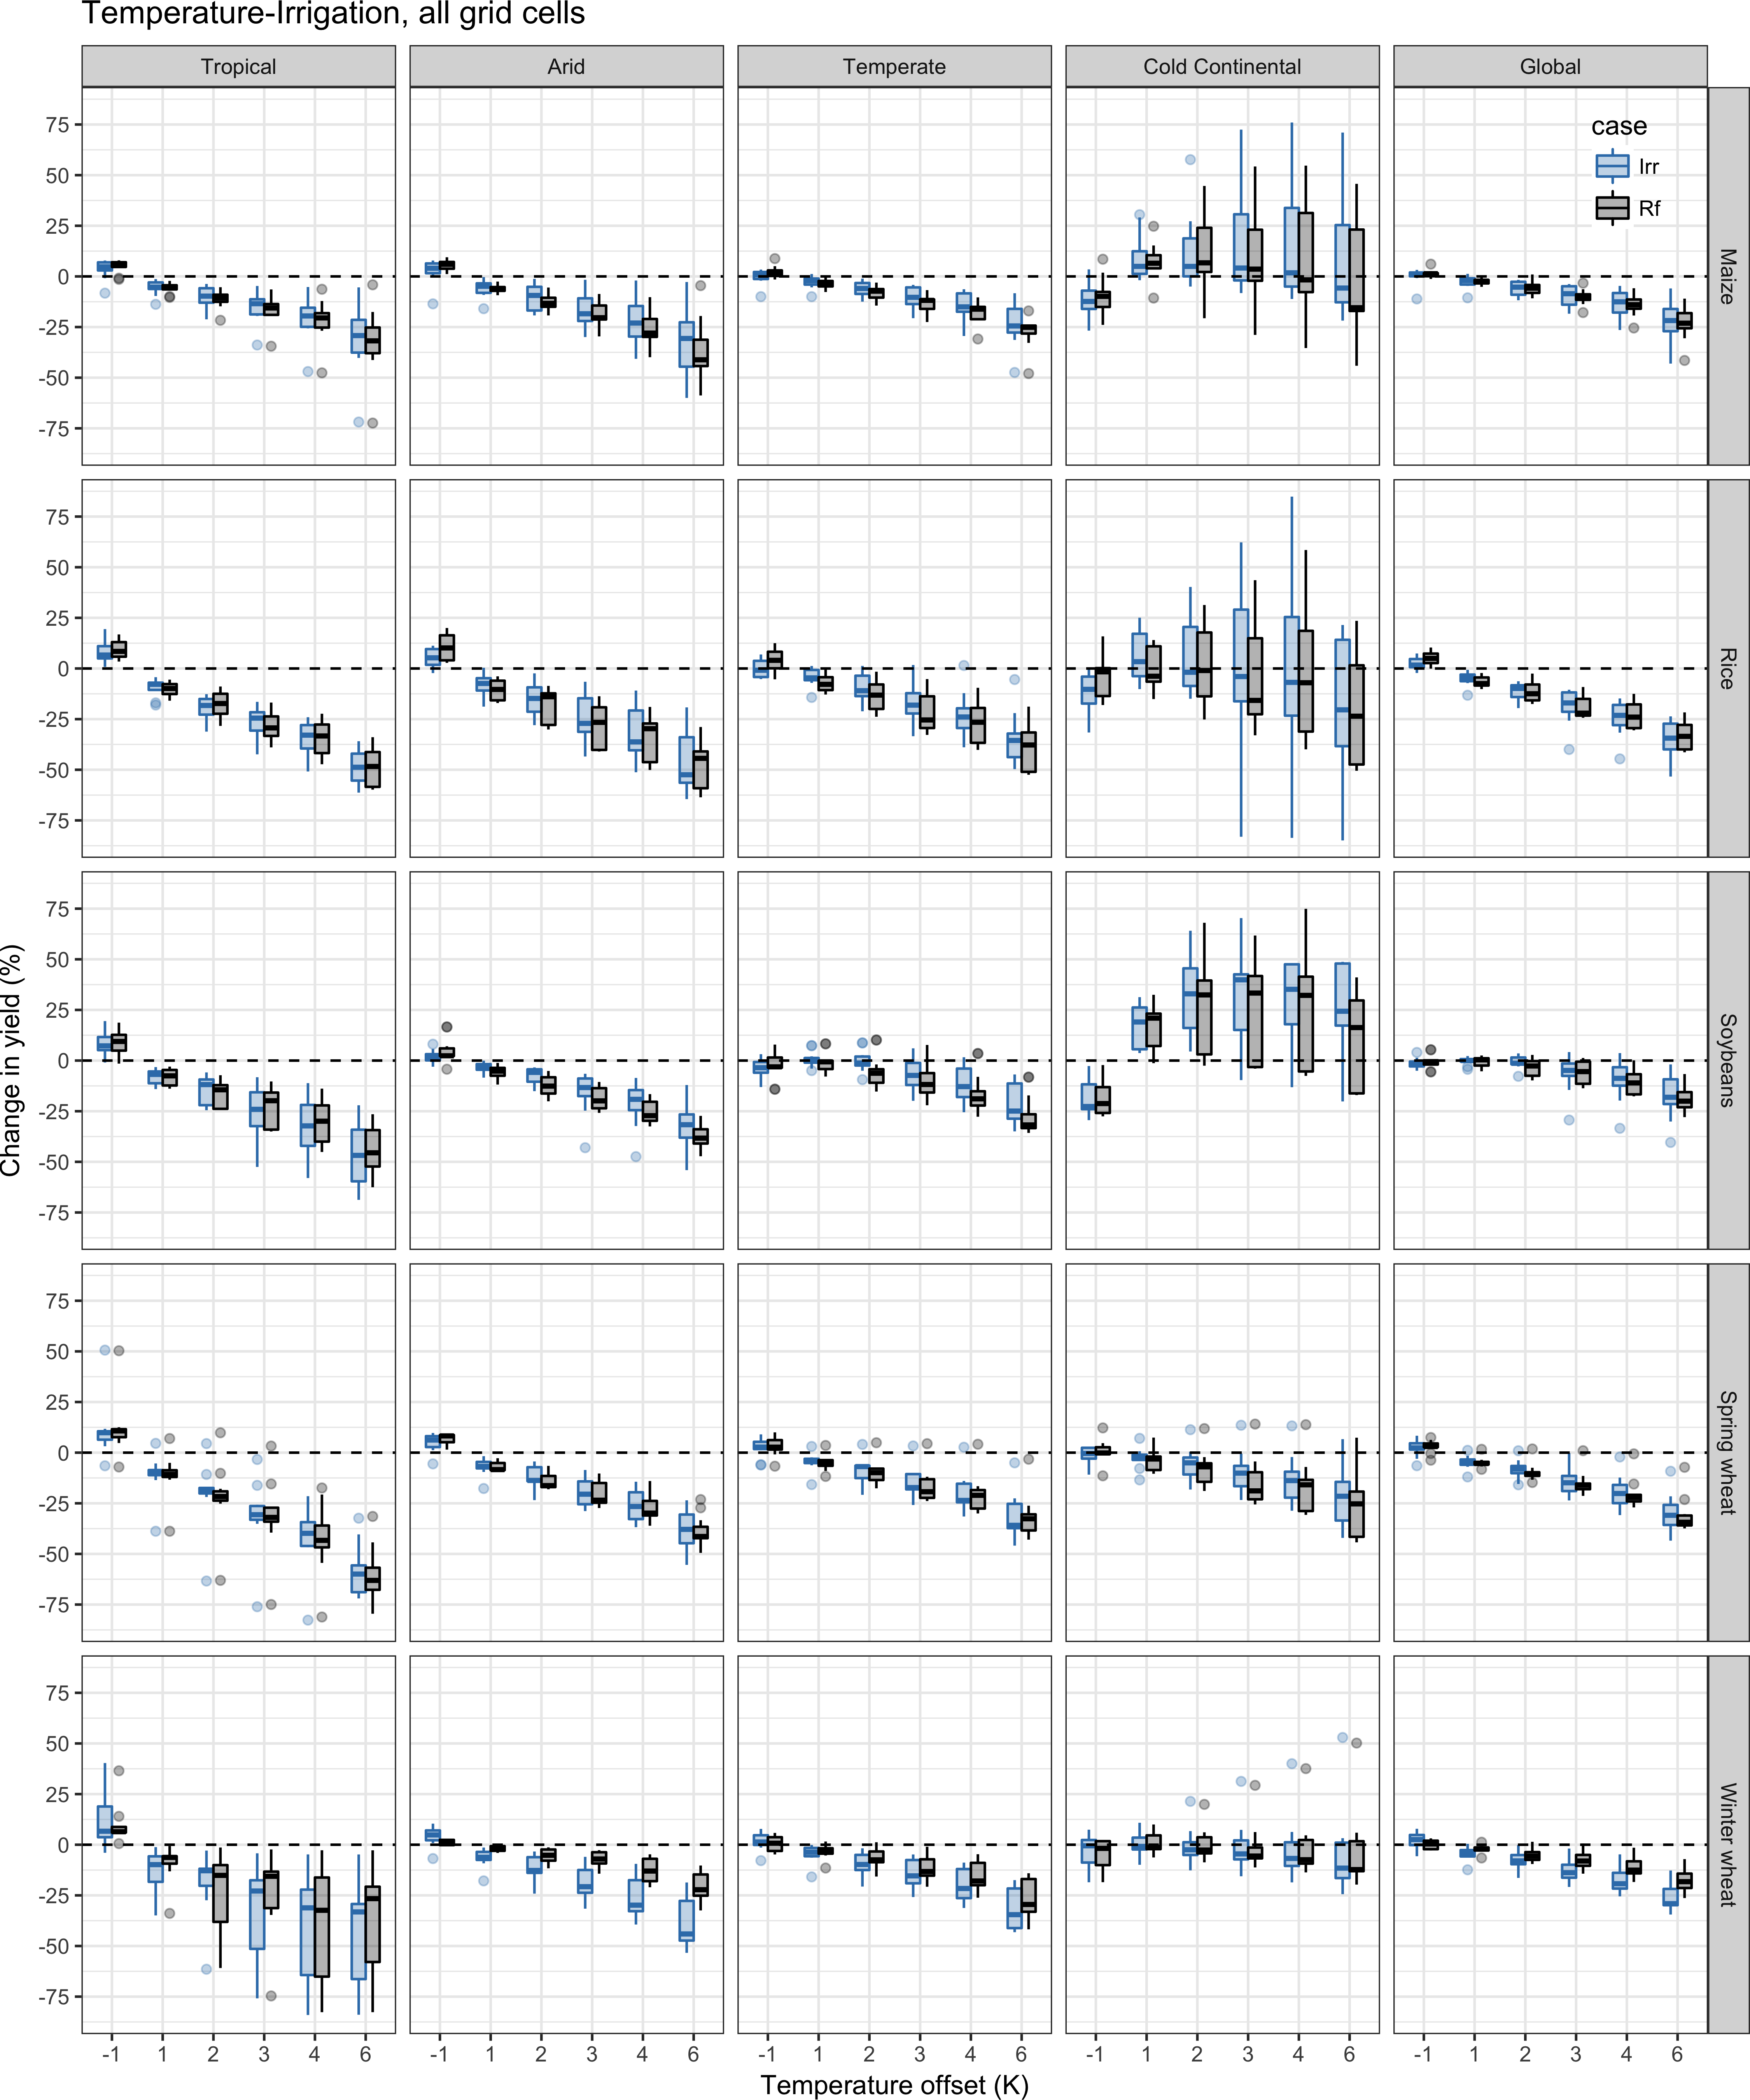
\includegraphics[width=\textwidth]{s_sim_CG_T_irr.png}
    \caption{Same as main Figure 5a for all crops. Irrigated crops compared to rainfed. Note that yield change for irrigated crops is from the irrigated baseline, which is typically higher than rainfed.}
    \label{fig:temp_irr}
\end{figure}

\begin{figure}[h!]
    \centering
    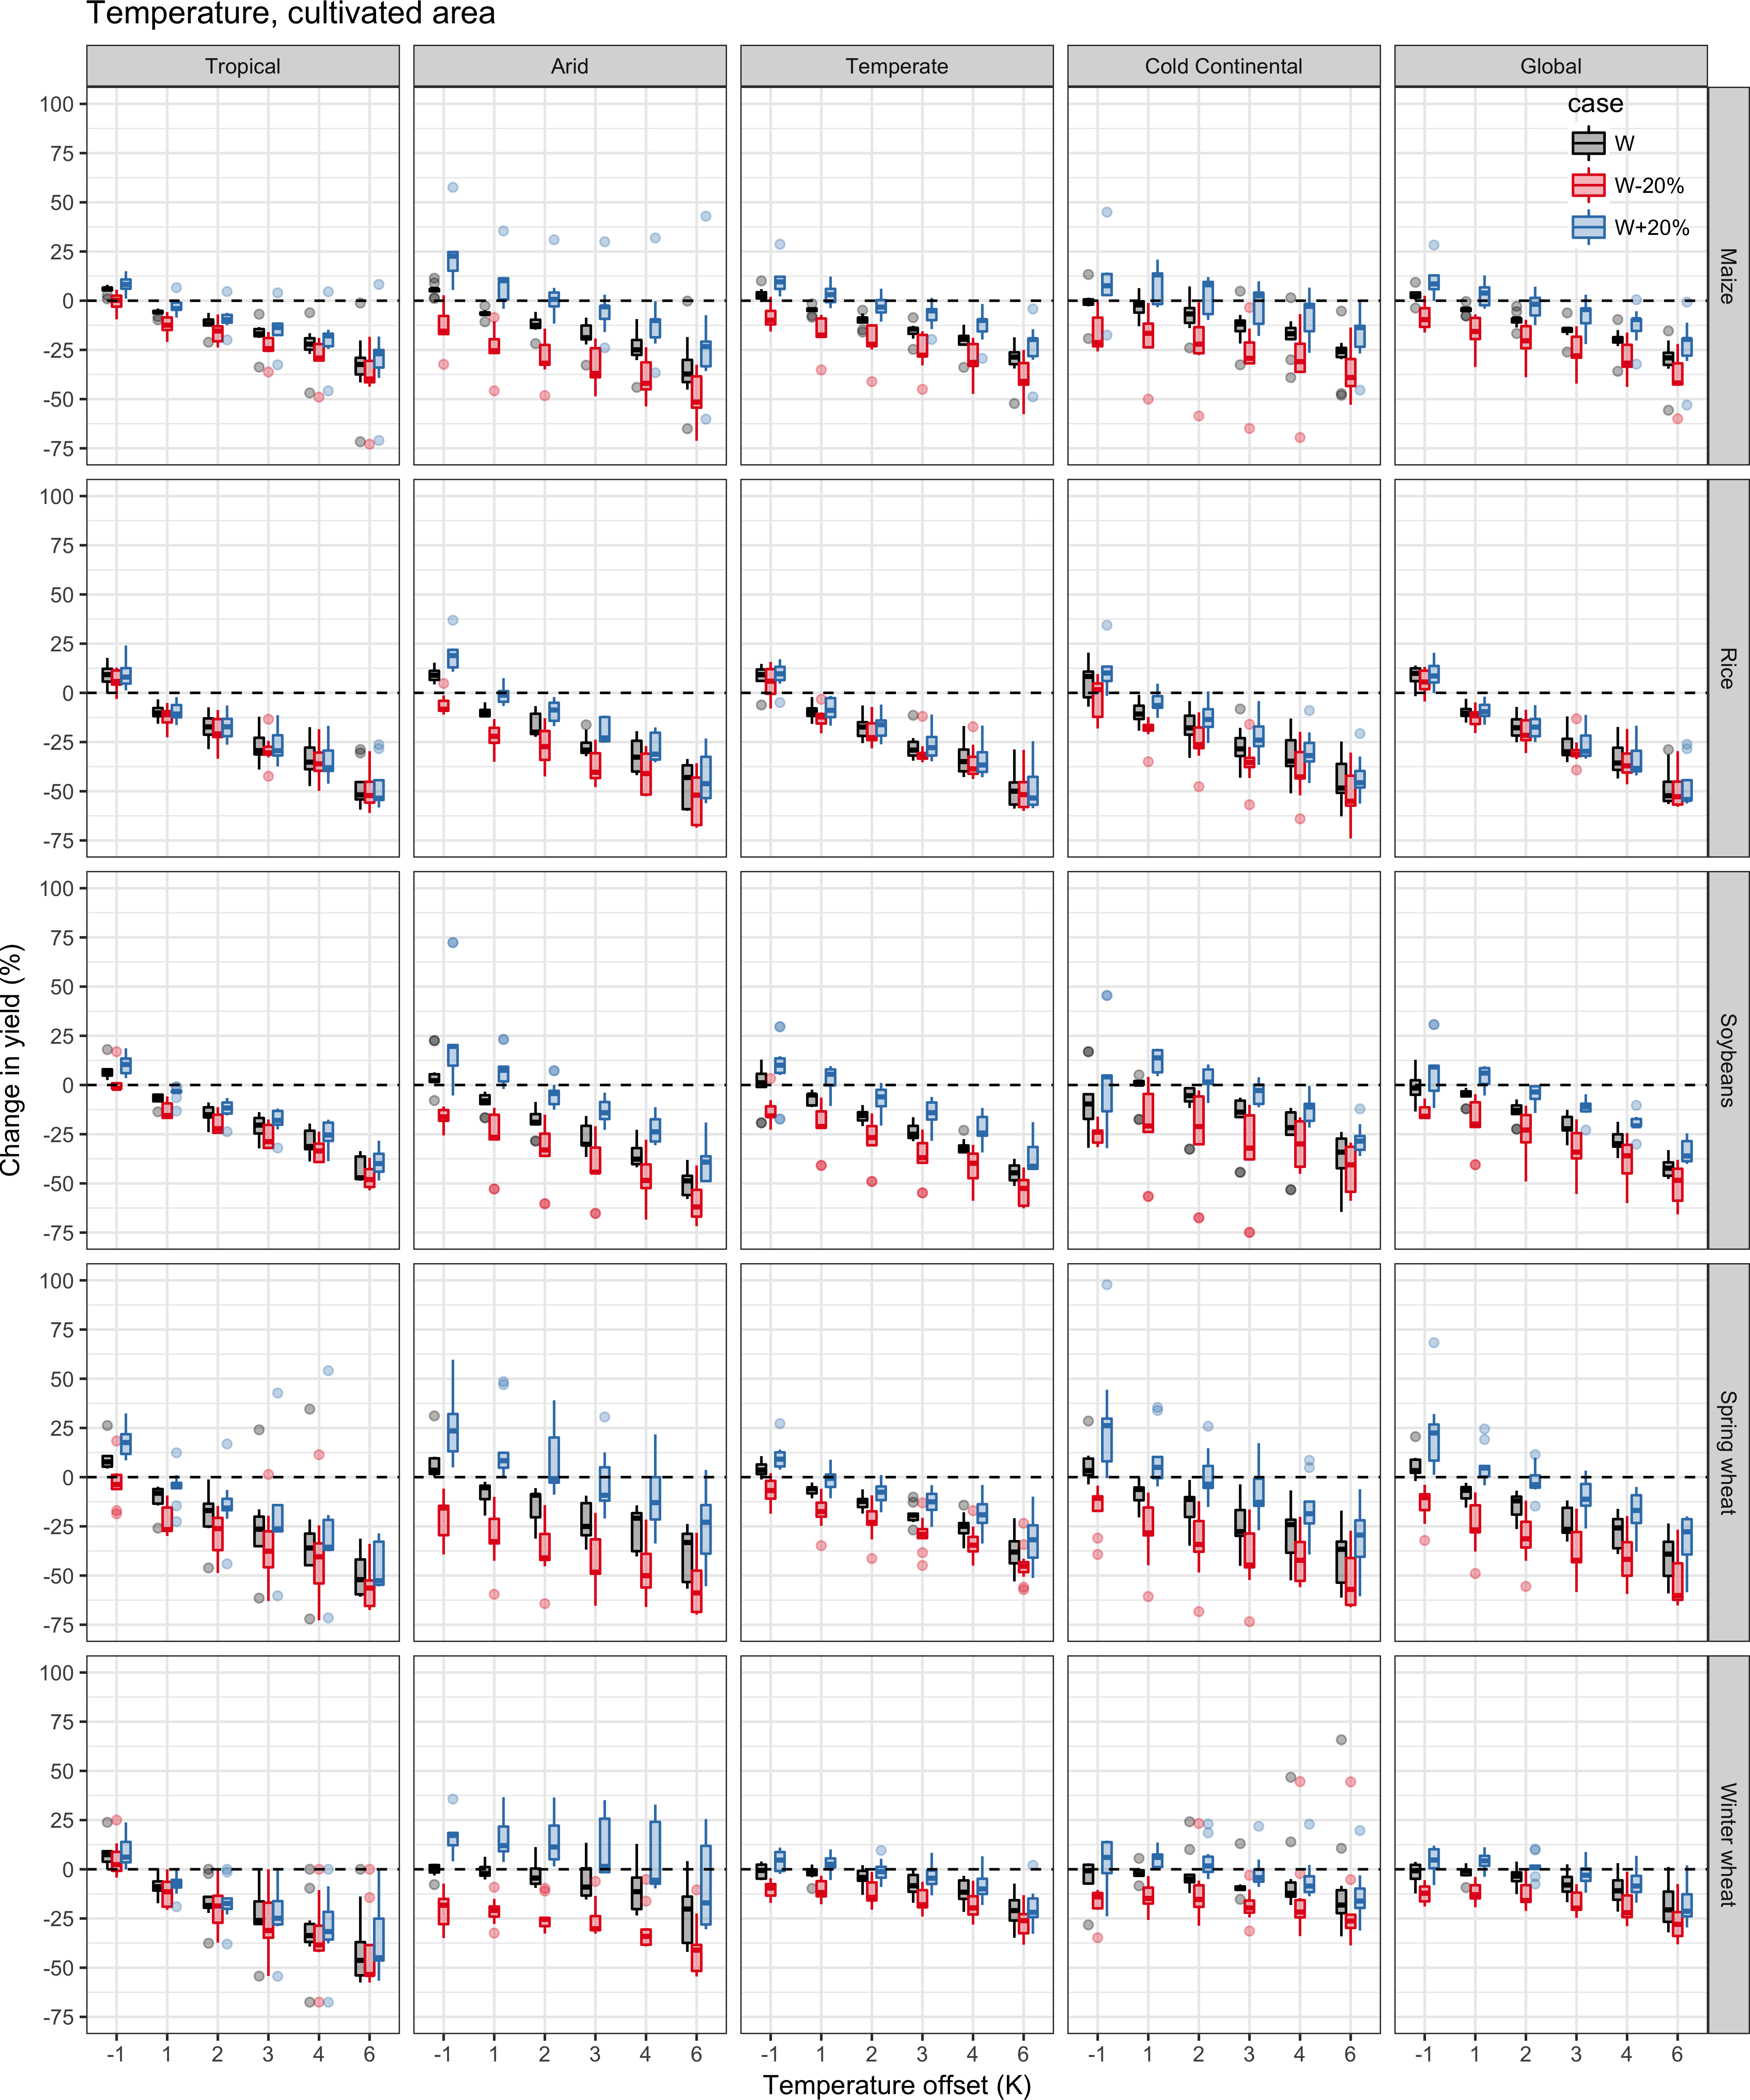
\includegraphics[width=\textwidth]{s_sim_CG_T_area.png}
    \caption{Same as main Figure 5a for all crops. Only over cultivated area.}
    \label{fig:temperautre}
\end{figure}

\begin{figure}[h!]
    \centering
    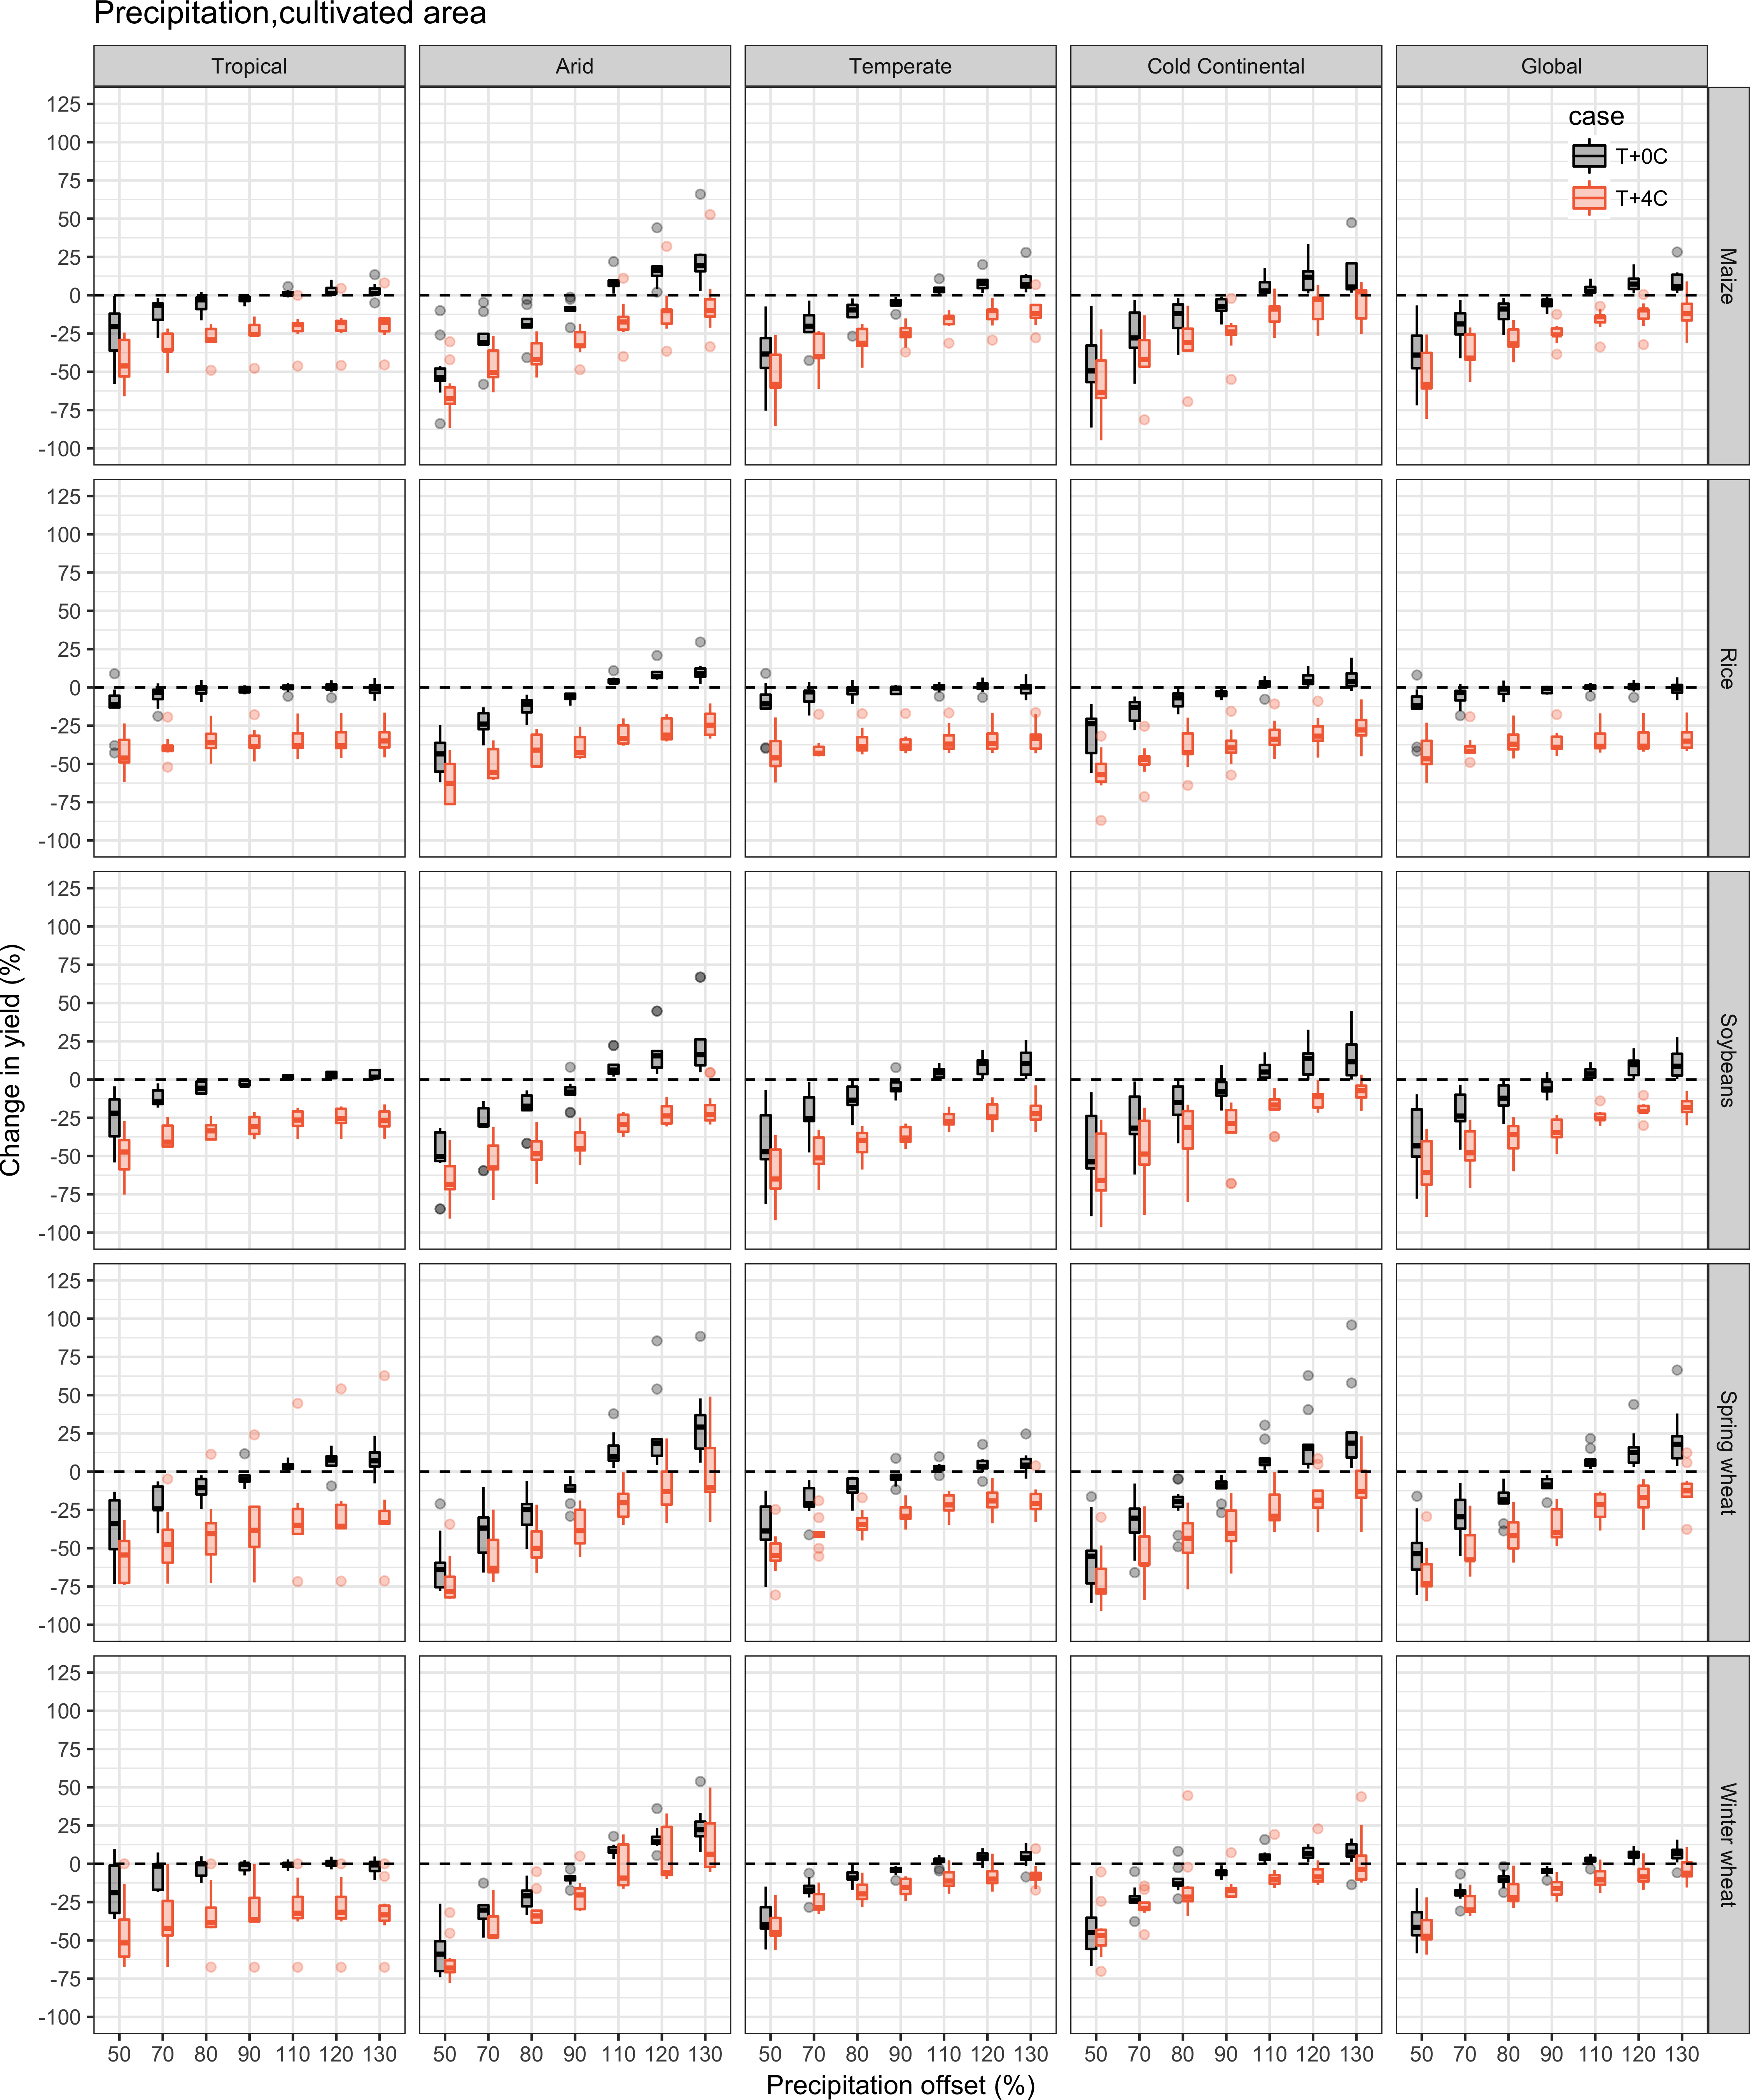
\includegraphics[width=\textwidth]{s_sim_CG_W_area.png}
    \caption{Same as main Figure 5b for all crops. Only over cultivated area.}
    \label{fig:water}
\end{figure}

\begin{figure}[h!]
    \centering
    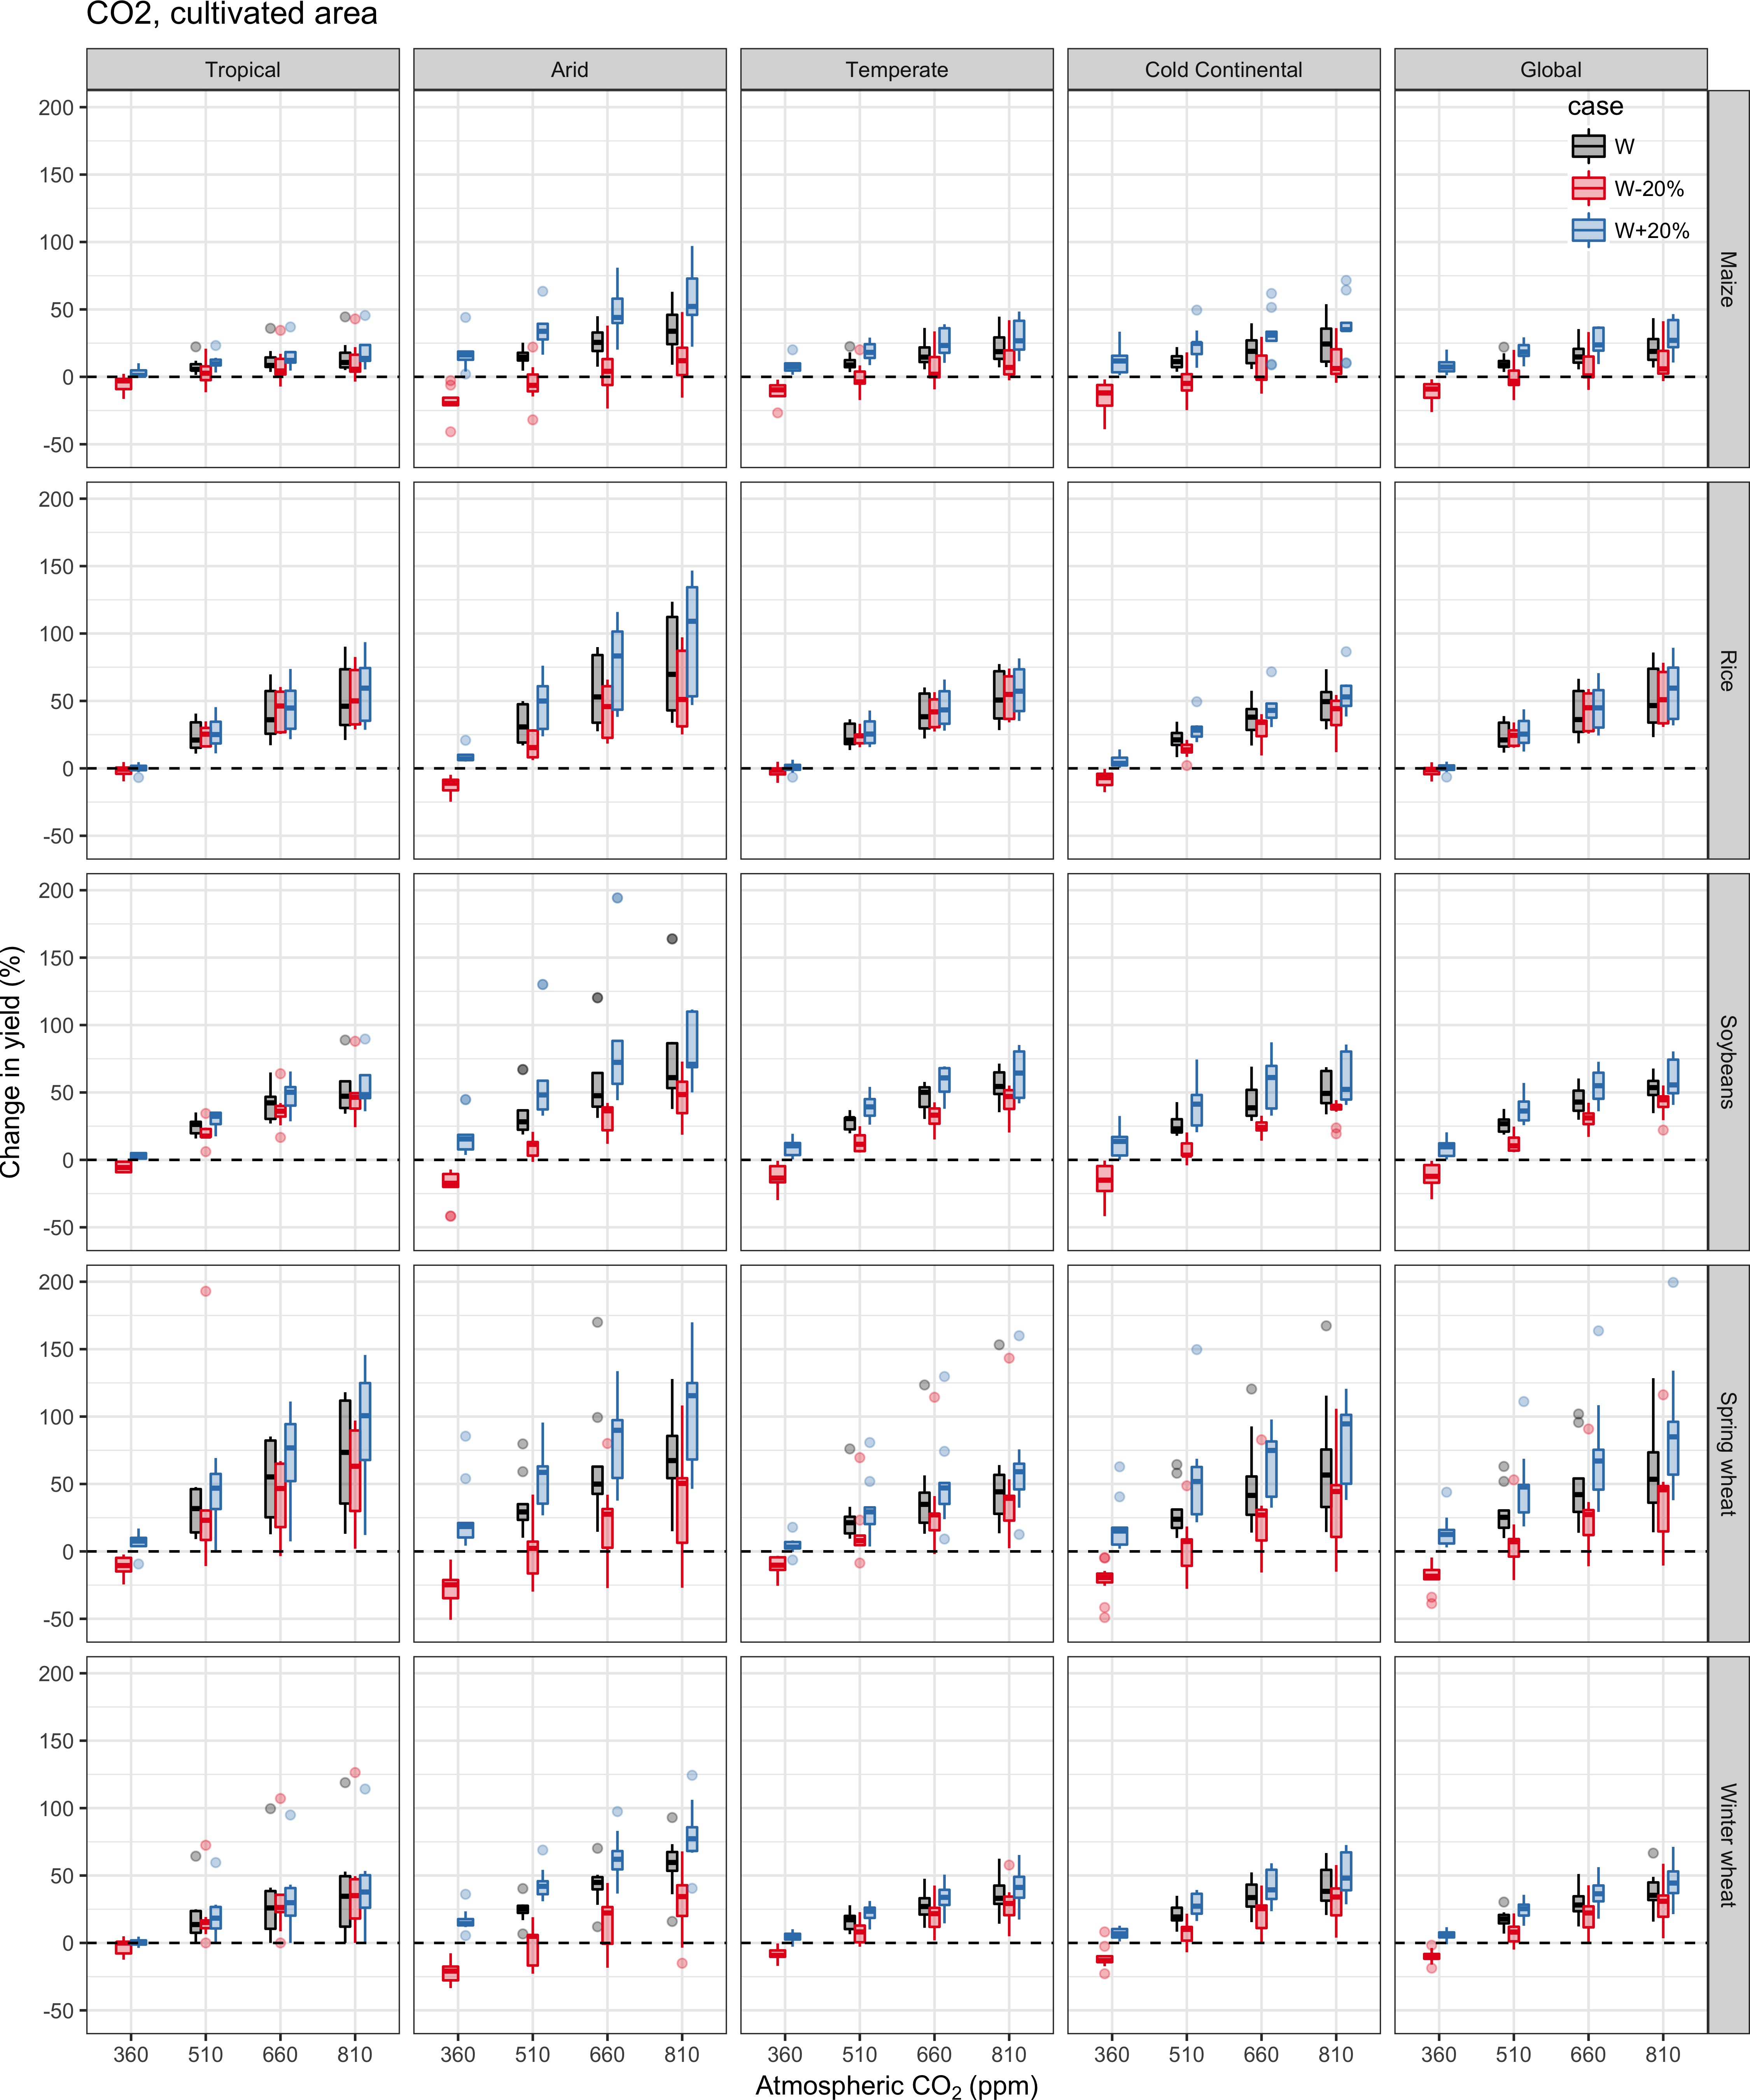
\includegraphics[width=\textwidth]{s_sim_CG_C_area.png}
    \caption{Same as main Figure 6a for all crops. Only over cultivated area.}
    \label{fig:carbon}
\end{figure}

\begin{figure}[h!]
    \centering
    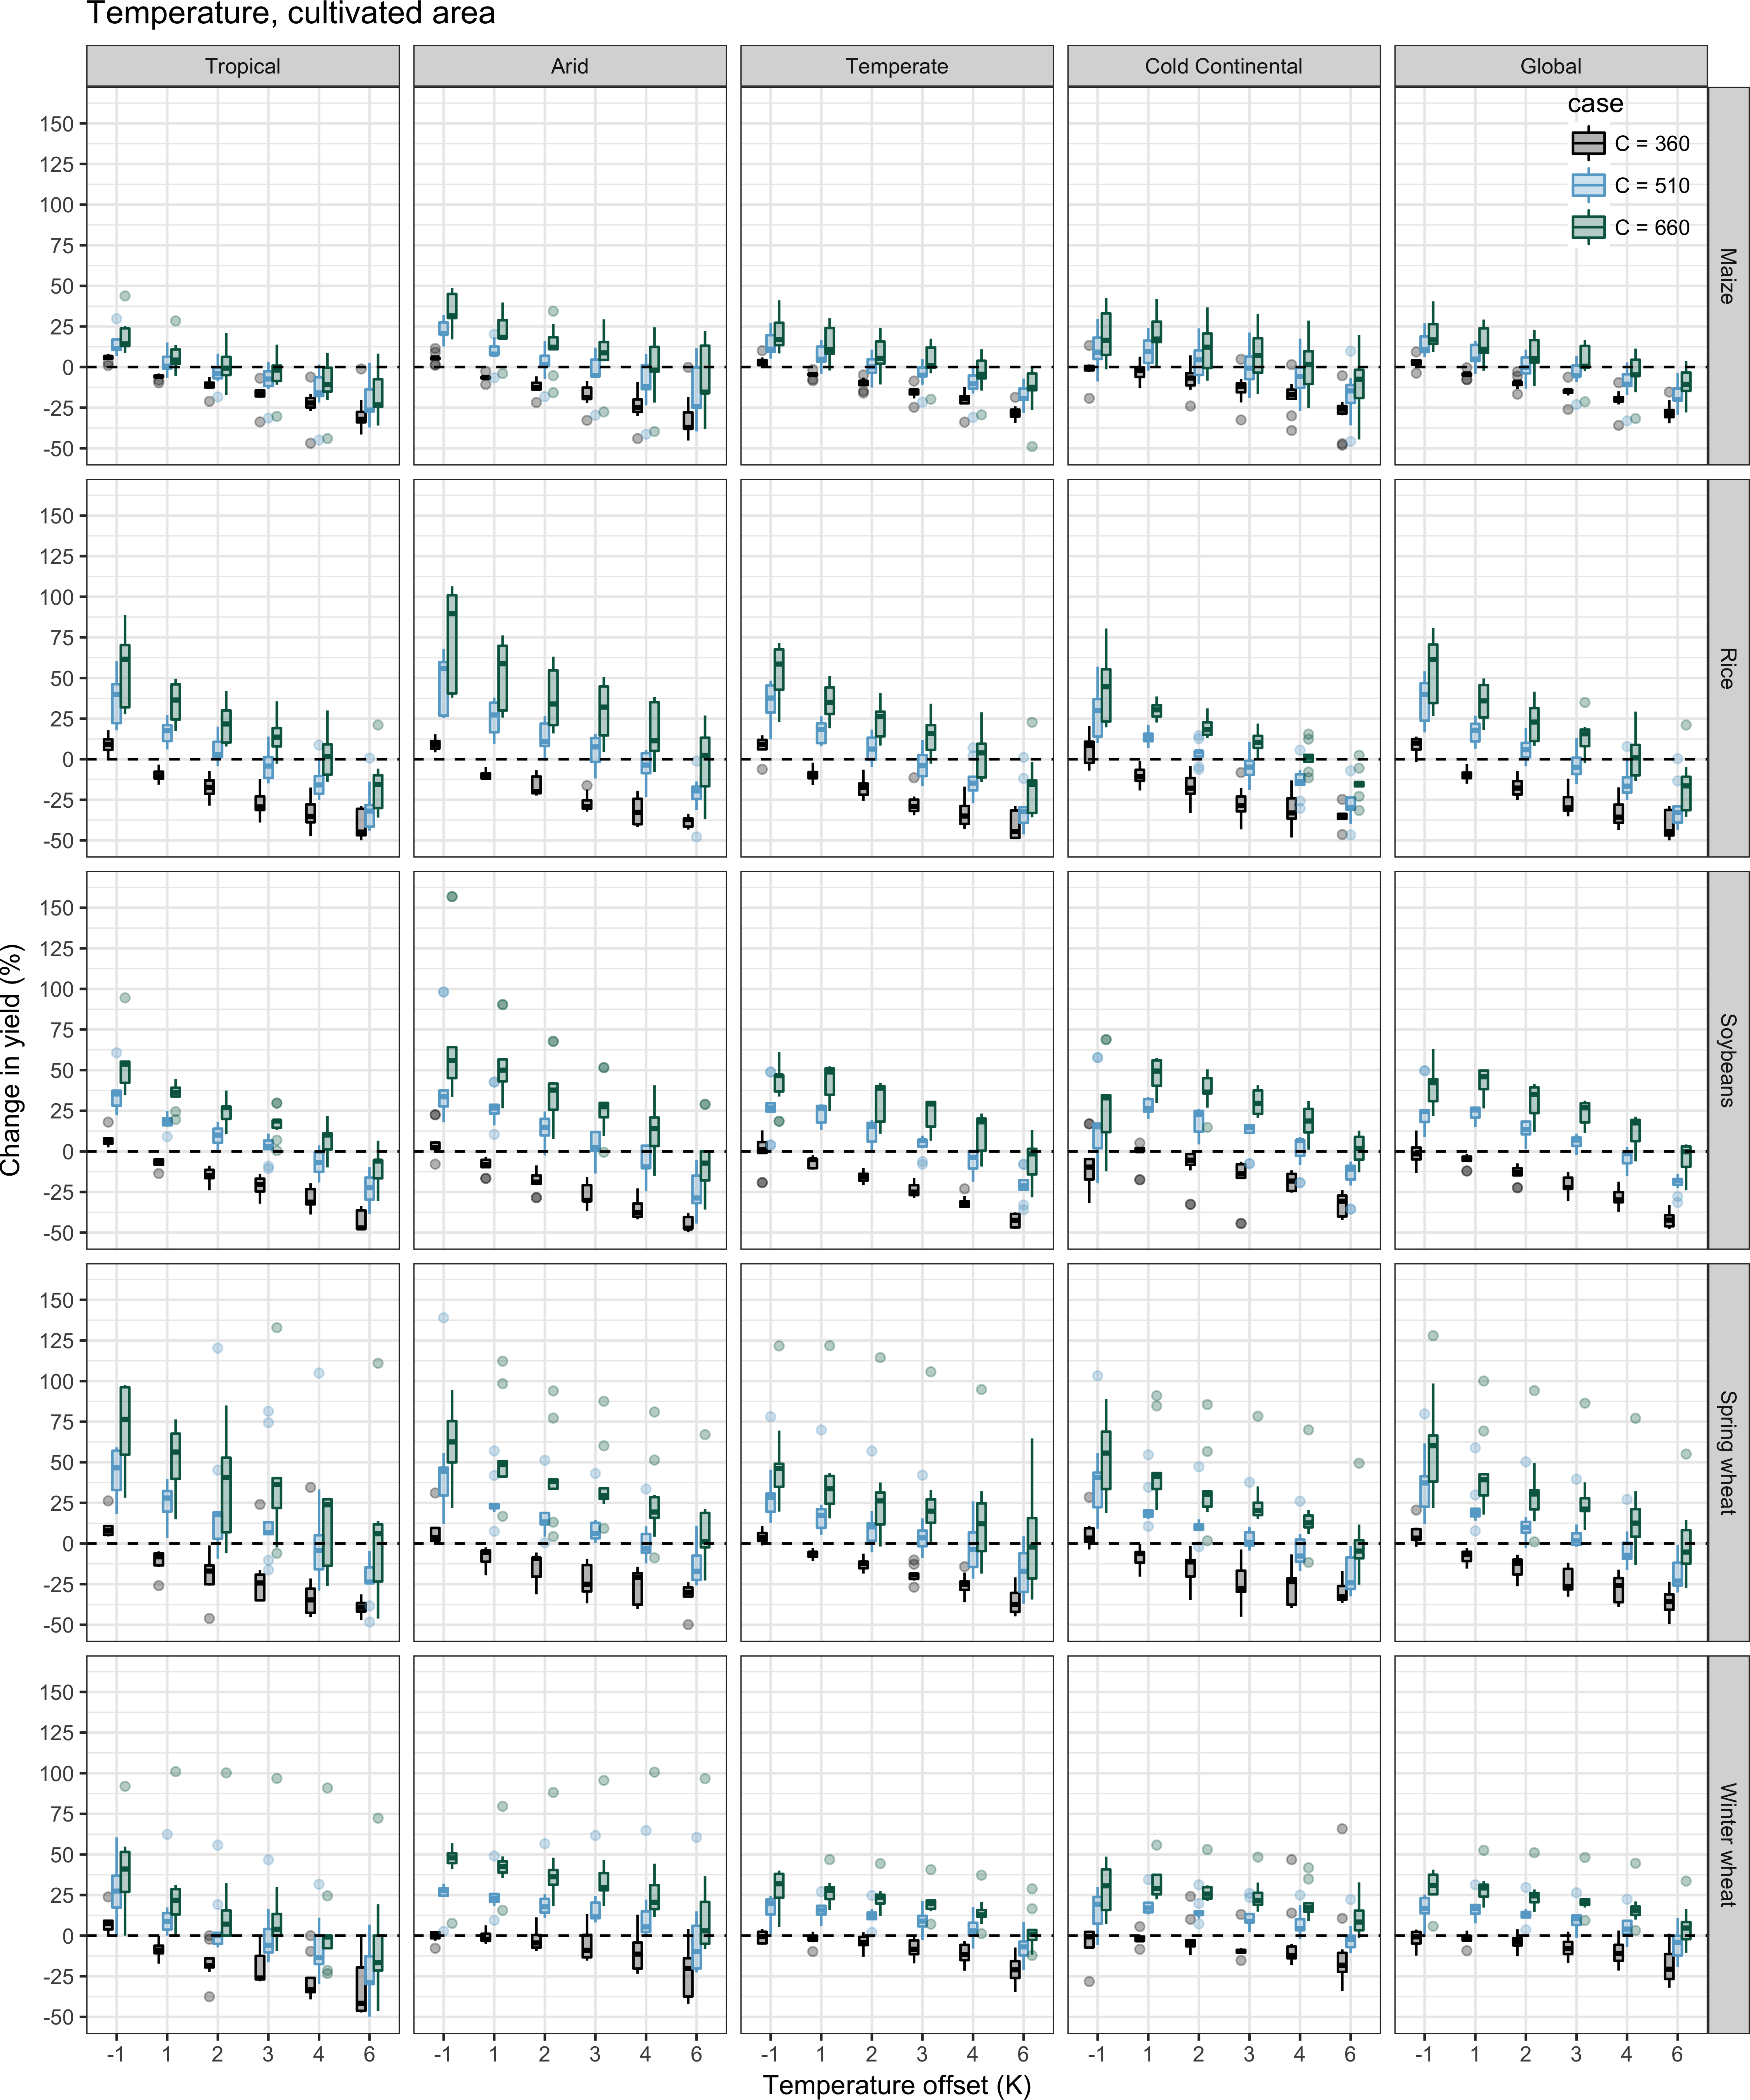
\includegraphics[width=\textwidth]{s_sim_CG_TC_area.png}
    \caption{Same as main Figure 6b for all crops. Only over cultivated area.}
    \label{fig:carbontemp}
\end{figure}

\begin{figure}[h!]
    \centering
    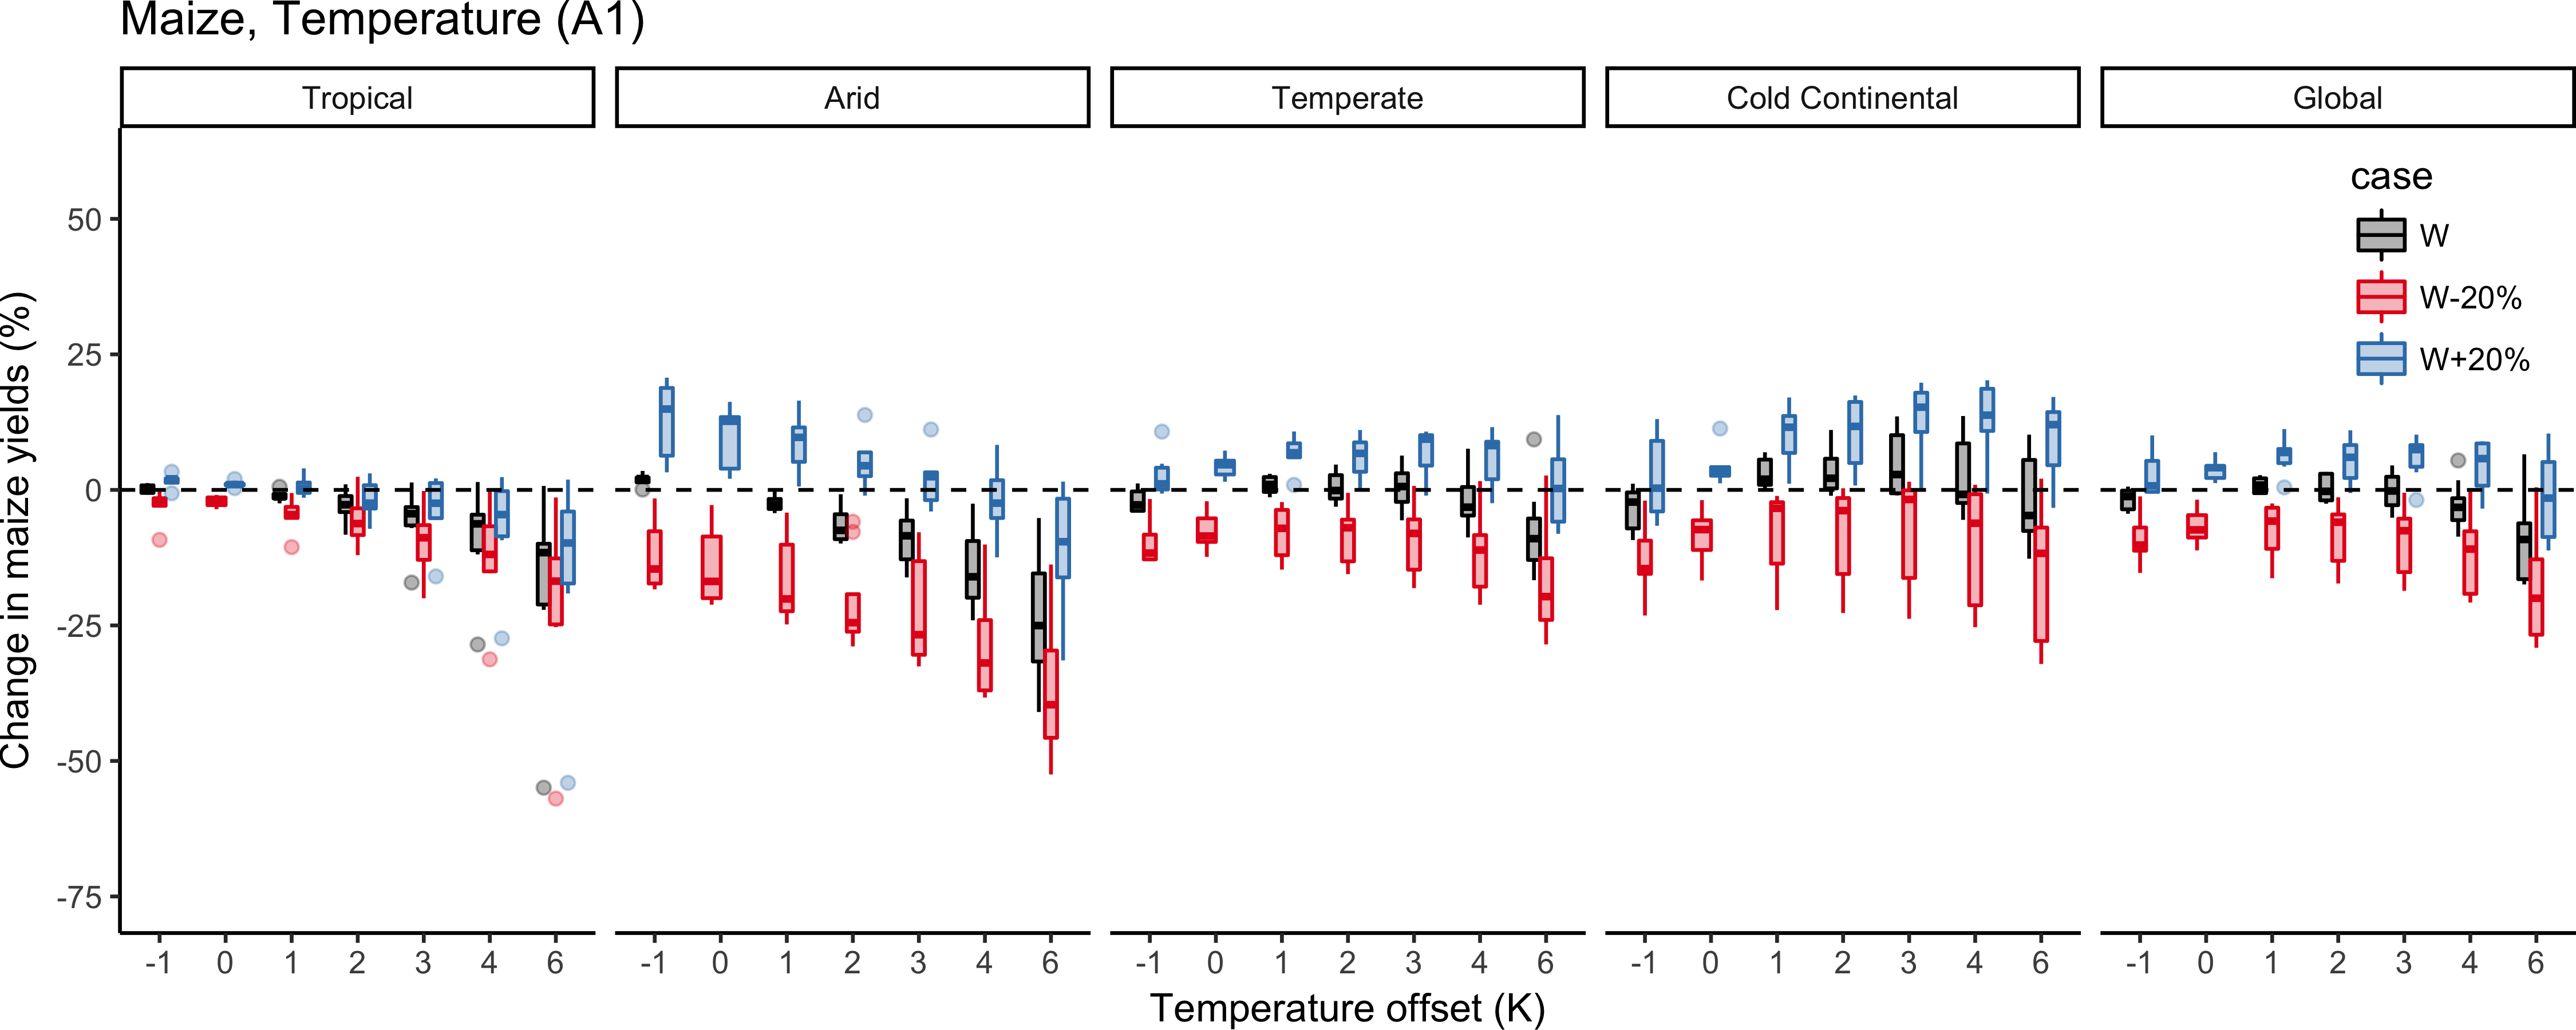
\includegraphics[width=\textwidth]{maize_sim_CG_T_A1.png}
    \caption{Same as main Figure 5a for except for A1 simulations where the growing season in held constant under warming.}
    \label{fig:carbontemp}
\end{figure}

\begin{figure}[h!]
    \centering
    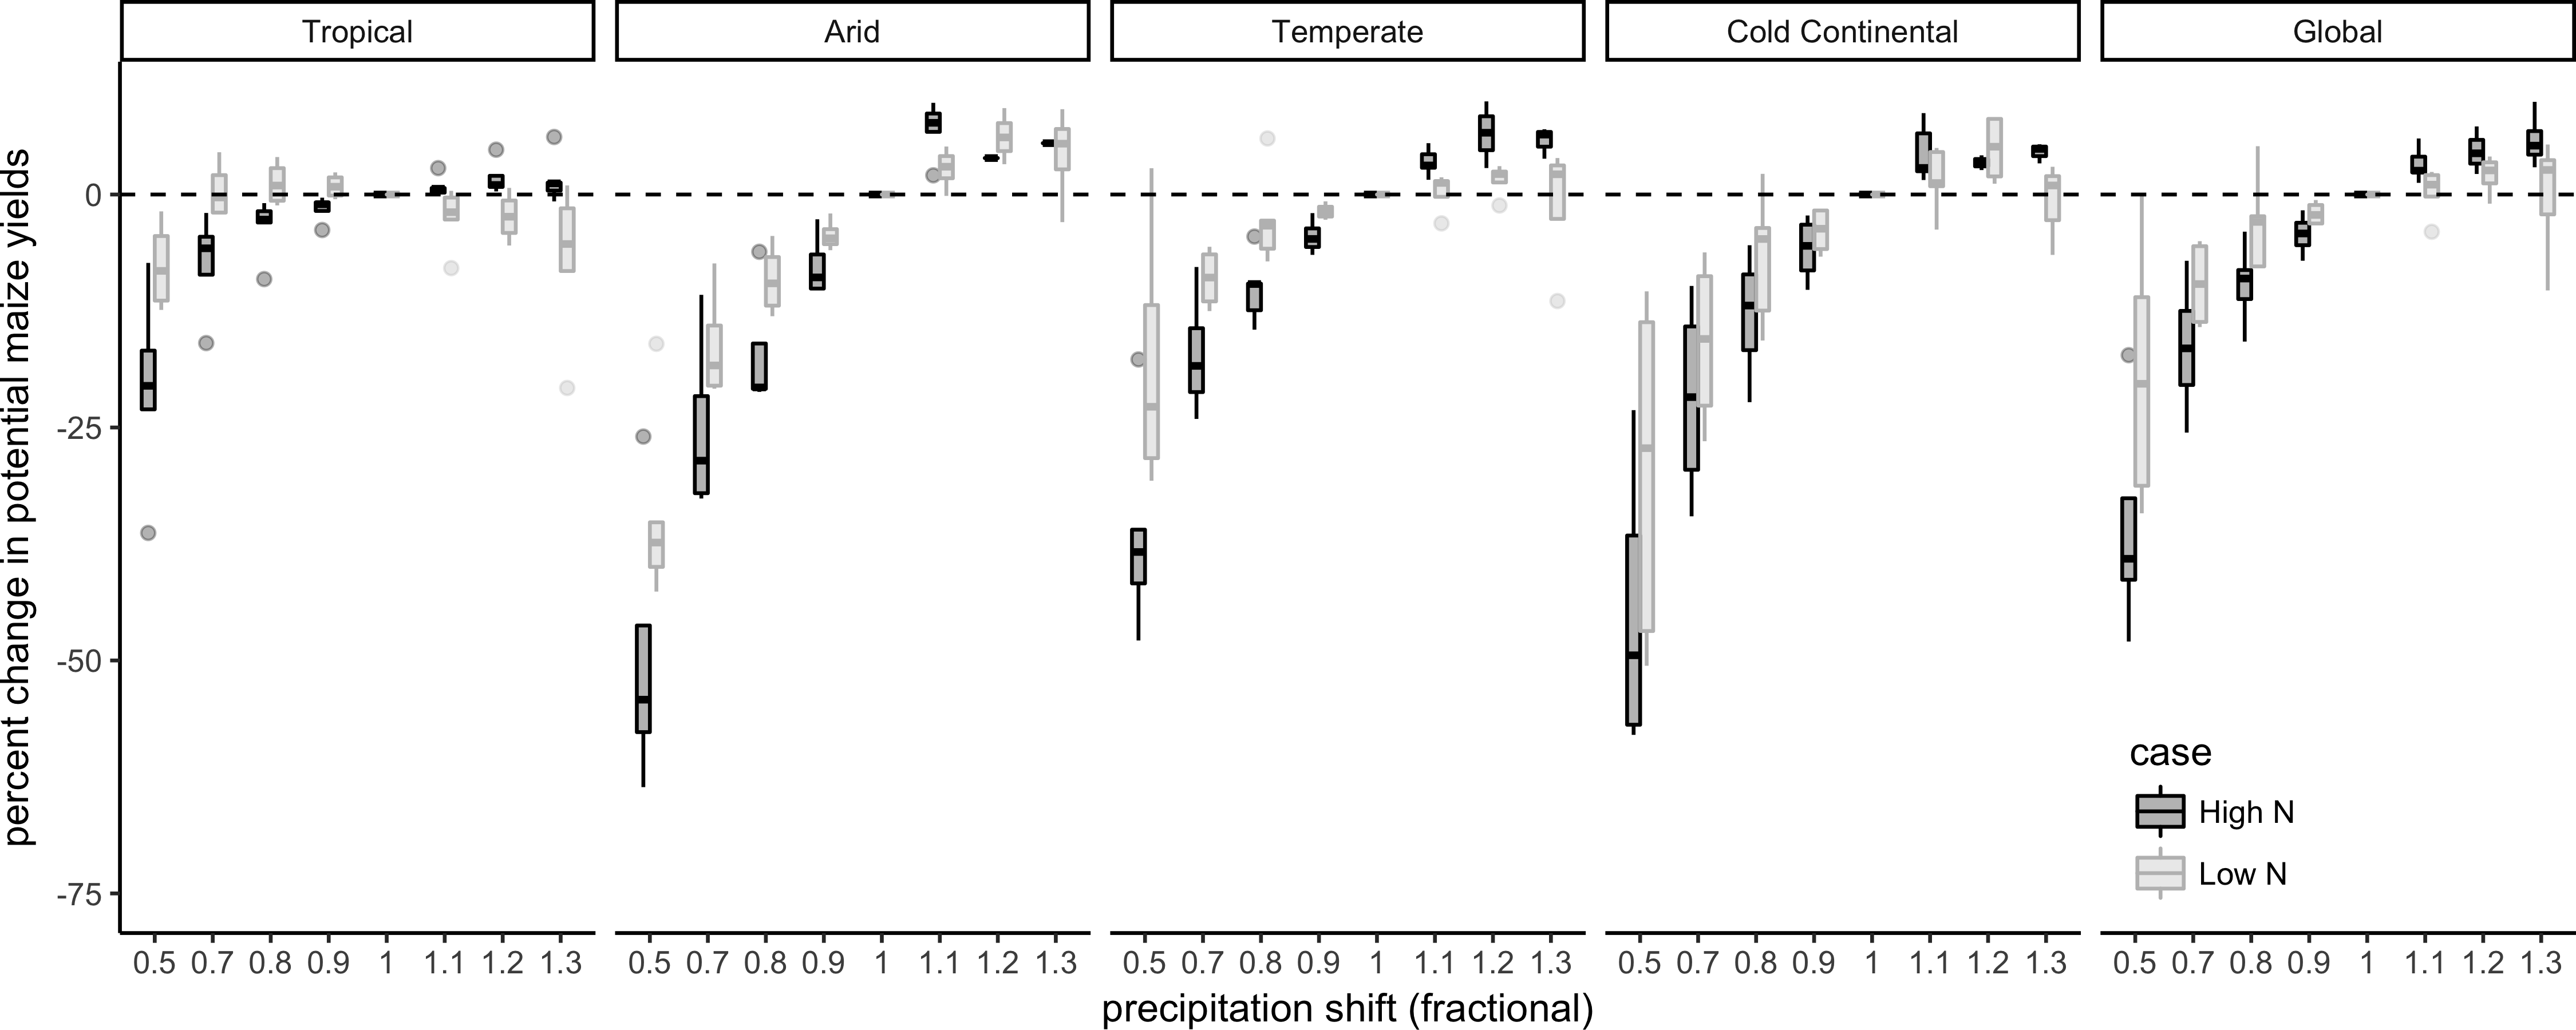
\includegraphics[width=\textwidth]{maize_sim_CG_N2.png}
    \caption{Same convention as main Figure 5b except for maize across the precipitation and nitrogen dimensions.}
    \label{fig:carbontemp}
\end{figure}

\begin{figure}[h!]
    \centering
    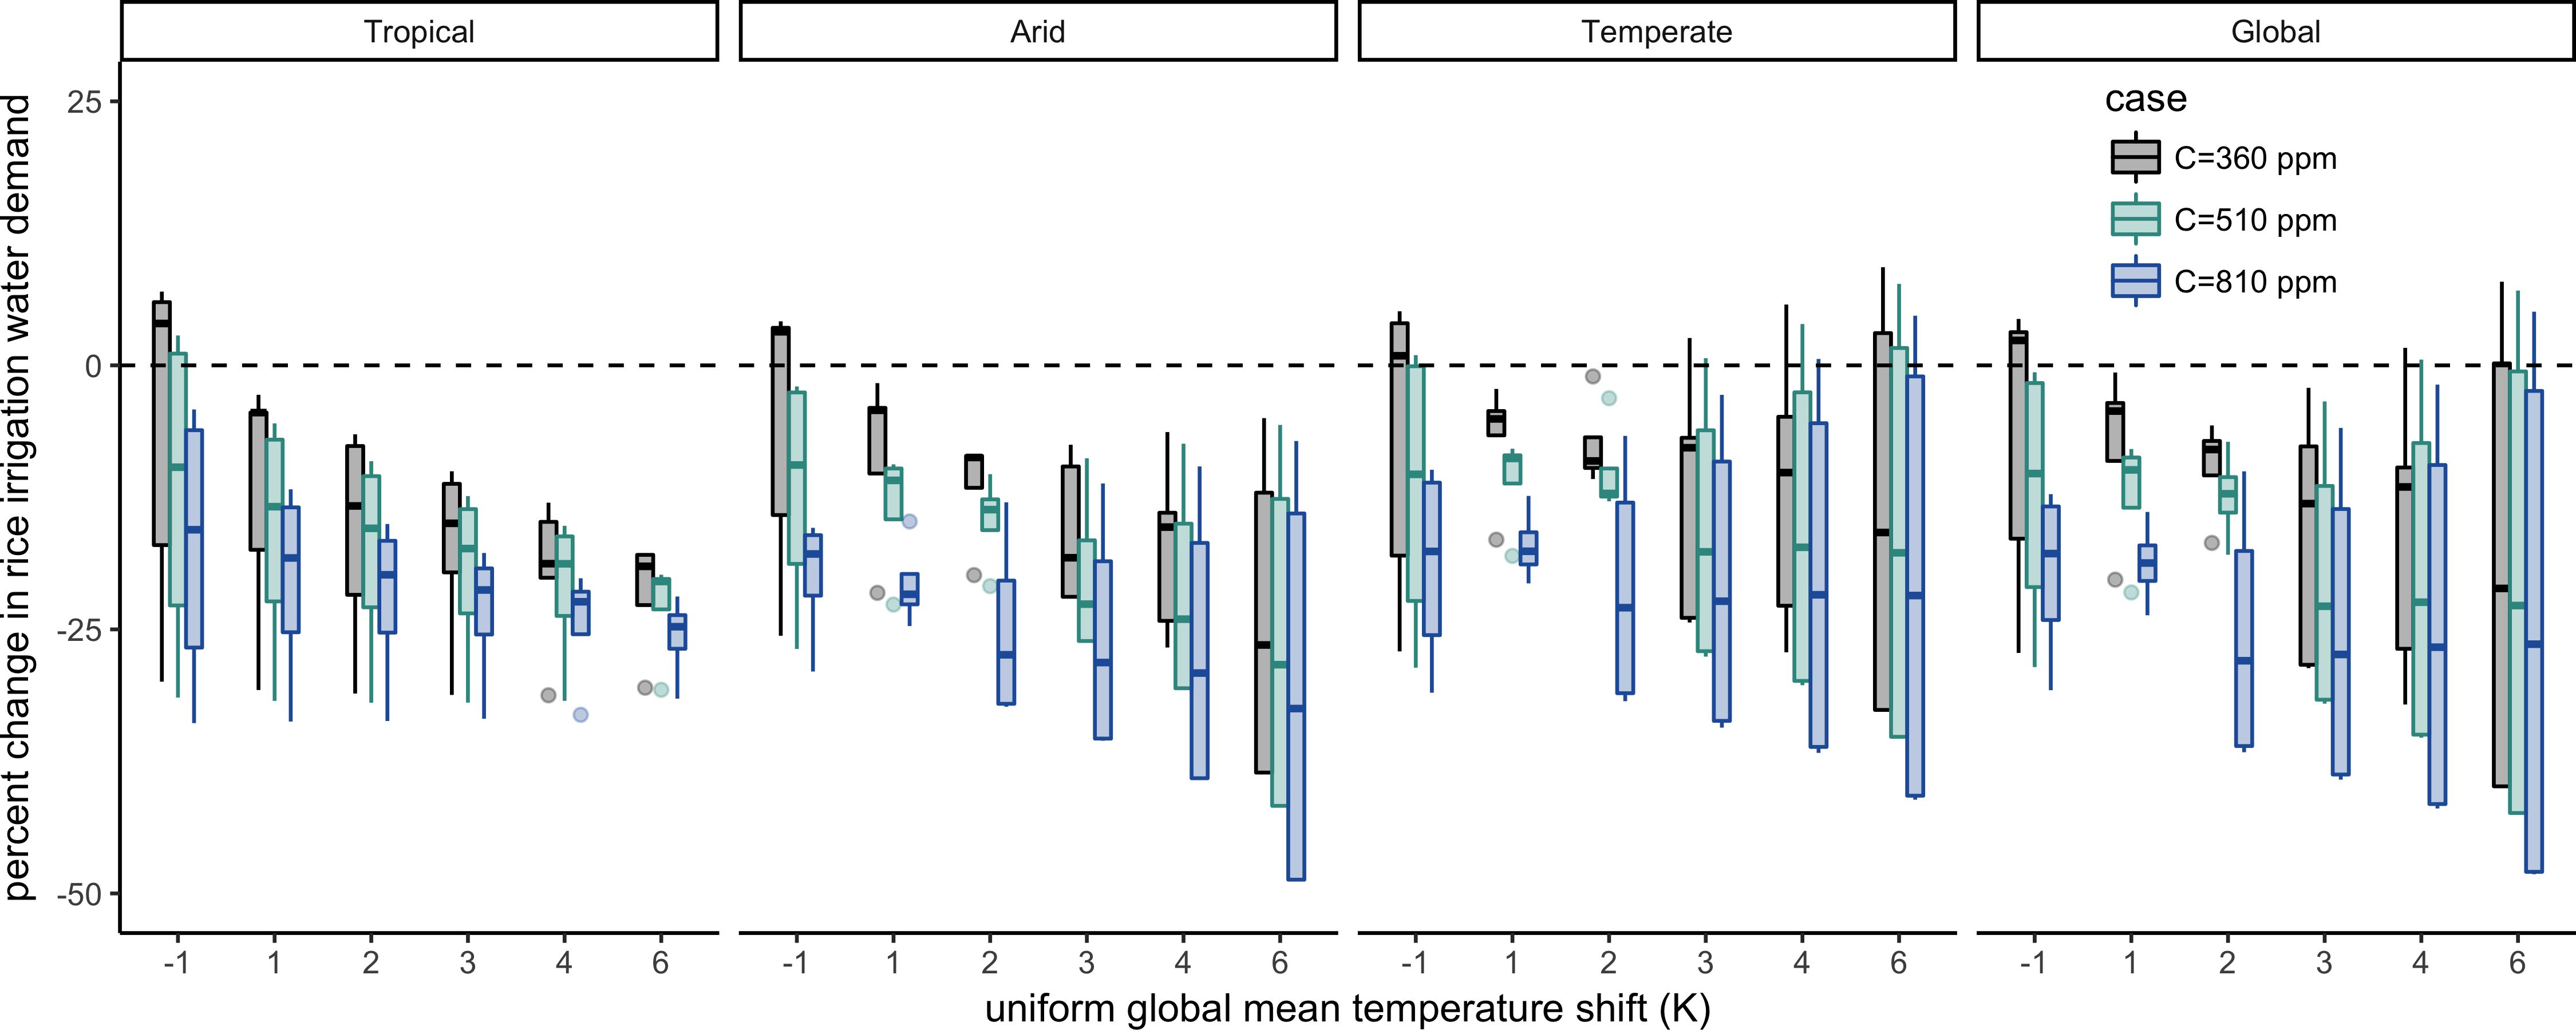
\includegraphics[width=\textwidth]{rice_sim_CG_irrwat.png}
    \caption{Same convention as main Figure 6b except for irrigation water demand instead of yield.}
    \label{fig:carbontemp}
\end{figure}




\end{document}


